\documentclass[10pt]{article}

%Math
\usepackage{amsmath}
\usepackage{amsfonts}
\usepackage{amssymb}
\usepackage{amsthm}
\usepackage{ulem}
\usepackage{stmaryrd} %f\UTF{00FC}r Blitz!

%PageStyle
\usepackage[ngerman]{babel} % deutsche Silbentrennung
\usepackage[utf8]{inputenc} 
\usepackage{fancyhdr, graphicx}
\usepackage[scaled=0.92]{helvet}
\usepackage{enumitem}
\usepackage{parskip}
\usepackage[a4paper,top=2cm]{geometry}
\setlength{\textwidth}{17cm}
\setlength{\oddsidemargin}{-0.5cm}
\usepackage{floatrow}

\newfloatcommand{capbtabbox}{table}[][] 

% Shortcommands
\newcommand{\Bold}[1]{\textbf{#1}} %Boldface
\newcommand{\Kursiv}[1]{\textit{#1}} %Italic
\newcommand{\T}[1]{\text{#1}} %Textmode
\newcommand{\Nicht}[1]{\T{\sout{$ #1 $}}} %Streicht Shit durch

%Arrows
\newcommand{\lra}{\leftrightarrow} 
\newcommand{\ra}{\rightarrow}
\newcommand{\la}{\leftarrow}
\newcommand{\lral}{\longleftrightarrow}
\newcommand{\ral}{\longrightarrow}
\newcommand{\lal}{\longleftarrow}
\newcommand{\Lra}{\Leftrightarrow}
\newcommand{\Ra}{\Rightarrow}
\newcommand{\La}{\Leftarrow}
\newcommand{\Lral}{\Longleftrightarrow}
\newcommand{\Ral}{\Longrightarrow}
\newcommand{\Lal}{\Longleftarrow}

\newcommand{\BN}{\mathfrak{B}} %Belegung
\newcommand{\RN}{\mathbb{R}} %Real Number
\newcommand{\NN}{\mathbb{N}} %Natural Number
\newcommand{\QN}{\mathbb{Q}} %Rational Number
\newcommand{\ZN}{\mathbb{Z}} %ganze Zahlen
\newcommand{\CN}{\mathbb{C}}

% Code listenings
\usepackage{color}
\usepackage{xcolor}
\usepackage{listings}
\usepackage{caption}
\DeclareCaptionFont{white}{\color{white}}
\DeclareCaptionFormat{listing}{\colorbox{gray}{\parbox{\textwidth}{#1#2#3}}}
\captionsetup[lstlisting]{format=listing,labelfont=white,textfont=white}
\lstdefinestyle{CStyle}{
 language=Java,
 basicstyle=\footnotesize\ttfamily, % Standardschrift
 numbers=left,               % Ort der Zeilennummern
 numberstyle=\tiny,          % Stil der Zeilennummern
 stepnumber=5,              % Abstand zwischen den Zeilennummern
 numbersep=5pt,              % Abstand der Nummern zum Text
 tabsize=2,                  % Groesse von Tabs
 extendedchars=true,         %
 breaklines=true,            % Zeilen werden Umgebrochen
 frame=b,         
 %commentstyle=\itshape\color{LightLime}, Was isch das? O_o
 %keywordstyle=\bfseries\color{DarkPurple}, und das O_o
 basicstyle=\footnotesize\ttfamily,
 stringstyle=\color[RGB]{42,0,255}\ttfamily, % Farbe der String
 keywordstyle=\color[RGB]{127,0,85}\ttfamily, % Farbe der Keywords
 commentstyle=\color[RGB]{63,127,95}\ttfamily, % Farbe des Kommentars
 showspaces=false,           % Leerzeichen anzeigen ?
 showtabs=false,             % Tabs anzeigen ?
 xleftmargin=17pt,
 framexleftmargin=17pt,
 framexrightmargin=5pt,
 framexbottommargin=4pt,
 showstringspaces=false      % Leerzeichen in Strings anzeigen ?        
}
\lstdefinestyle{JavaStyle}{
 language=Java,
 basicstyle=\footnotesize\ttfamily, % Standardschrift
 numbers=left,               % Ort der Zeilennummern
 numberstyle=\tiny,          % Stil der Zeilennummern
 stepnumber=5,              % Abstand zwischen den Zeilennummern
 numbersep=5pt,              % Abstand der Nummern zum Text
 tabsize=2,                  % Groesse von Tabs
 extendedchars=true,         %
 breaklines=true,            % Zeilen werden Umgebrochen
 frame=b,         
 %commentstyle=\itshape\color{LightLime}, Was isch das? O_o
 %keywordstyle=\bfseries\color{DarkPurple}, und das O_o
 basicstyle=\footnotesize\ttfamily,
 stringstyle=\color[RGB]{42,0,255}\ttfamily, % Farbe der String
 keywordstyle=\color[RGB]{127,0,85}\ttfamily, % Farbe der Keywords
 commentstyle=\color[RGB]{63,127,95}\ttfamily, % Farbe des Kommentars
 showspaces=false,           % Leerzeichen anzeigen ?
 showtabs=false,             % Tabs anzeigen ?
 xleftmargin=17pt,
 framexleftmargin=17pt,
 framexrightmargin=5pt,
 framexbottommargin=4pt,
 showstringspaces=false      % Leerzeichen in Strings anzeigen ?        
}
%Config
\renewcommand{\headrulewidth}{0pt}
\setlength{\headheight}{15.2pt}

%Metadata
\fancyfoot[C]{If you use this documentation for a exam, you should offer a beer to the authors!}
\title{
	\vspace{5cm}
	Bildverarbeitung
}
\author{Jan Fässler}
\date{5. Semester (HS 2013)}


% hier beginnt das Dokument
\begin{document}

% Titelbild
\maketitle
\thispagestyle{fancy}

\newpage

% Inhaltsverzeichnis
\pagenumbering{Roman}
\tableofcontents	  	

\newpage
\setcounter{page}{1}
\pagenumbering{arabic}

\section{Einführung}
\subsection{Elektromagnetische Strahlung}
\begin{description}
	\item[Wellenlänge] \hfill \\
		$\lambda = \frac{c}{f}$ $[m]$, mit $c =$ Lichtgeschwindigkeit und $f =$ Frequenz
	\item[Energie der elektromagnetischen Strahlung] \hfill \\
		$E=h*f$ $[eV]$, mit $h=6.626*10^{-34}$ Js $= 4.136 * 10^{-15}$ eVs 
\end{description}
\begin{center}
	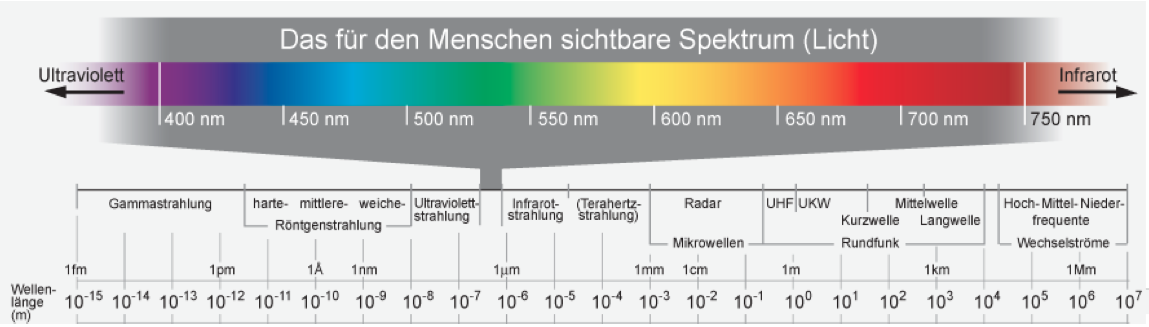
\includegraphics[scale=0.35]{lichtspektrum.png}
\end{center}

\subsection{Sensor-Arrays}
\subsubsection*{Funktionsprinzip}
\begin{itemize}
	\item Ladungen werden in einem Kondensator gesammelt
	\item die Ladungsmenge ist proportional zur eingestrahlten Lichtmenge, wenn rechtzeitig ausgelesen wird, bevor die Leerlaufspannung der Fotodiode erreicht ist
\end{itemize}
\subsubsection*{CCD}
\begin{itemize}
	\item Zeilen werden der Reihe nach ausgelesen
	\item pro Zeile werden die Ladungen serialisiert
	\item alle Ladungsmengen werden durch einen einzigen Ausleseverstärker geleitet
\end{itemize}
\subsubsection*{CMOS}
\begin{itemize}
	\item zu jeder Fotodiode gehört ein eigener Verstärker, welcher die Kondensatorspannung dem Analogsignalprozessor direkt zur Verfügung stellt
\end{itemize}

\subsection{Farbbilderzeugung}
\subsubsection*{Bayer-Maske}
\begin{center}
	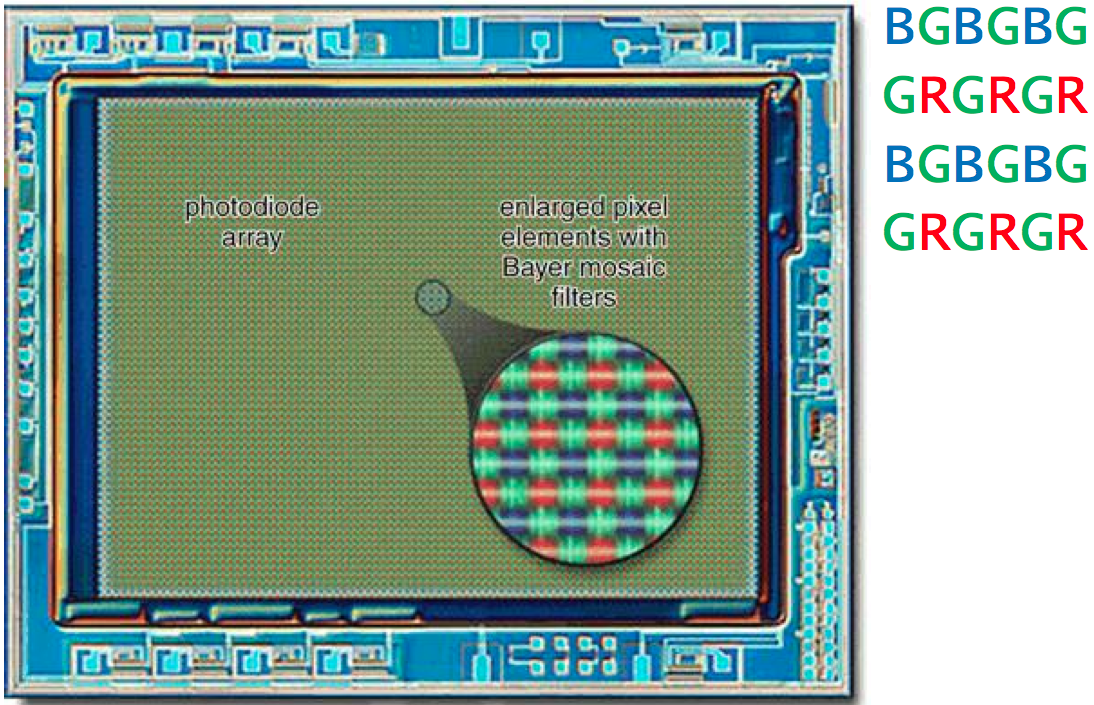
\includegraphics[scale=0.15]{bayer-maske.png} 
\end{center}
\subsubsection*{Andere}
\begin{tabular}{l l l}
	\textbf{Foveon} & \textbf{Filterrad mit RGB-Filter} & \textbf{Spektralzerlegung} \\
	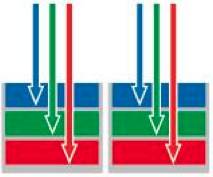
\includegraphics[scale=0.7]{foveon.png} & 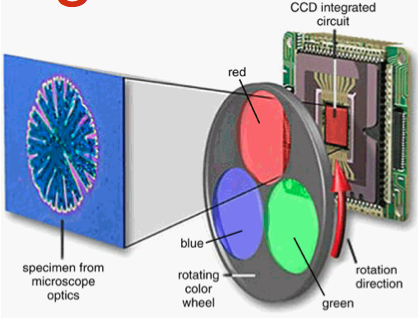
\includegraphics[scale=0.4]{Filterrad-mit-RGB-Filter.png} & 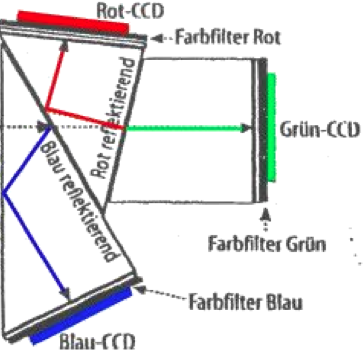
\includegraphics[scale=0.4]{spektralzerlegung.png}
\end{tabular}

\subsection{Digitales Rasterbild}
Entstehung eines digitalen Rasterbildes
\begin{enumerate}
	\item \textbf{räumliche Abtastung} \\
		Übergang von einer räumlichen zu einer diskreten Lichtverteilung durch Geometrie des Aufnahmesensors (z.B. CCD-Chip)
	\item \textbf{zeitliche Abtastung} \\
		Steuerung der Zeit, über die die Lichtmessung stattfindet
	\item \textbf{Quantisierung der Pixelwerte}\\
		gemessene Lichtwerte werden auf eine endliche Menge von Zahlenwerten abgebildet
\end{enumerate}	

\subsection{Raster- vs. Vektordaten}
\subsubsection*{Rasterbilder}
\begin{itemize}
	\item regelmässige Matrix (mit diskreten Koordinaten) von Pixelwerten
	\item typische Formate: BMP, JFIF, TIFF, PNG, PGF usw.
\end{itemize}
\subsubsection*{Vektorgrafiken}
\begin{itemize}
	\item geometrische Beschreibung mit kontinuierlichen Koordinaten
	\item Rasterung (falls notwendig) erfolgt erst bei der Ausgabe
	\item typische Formate: SVG, DXF usw.
\end{itemize}
\subsubsection*{Metaformate}
\begin{itemize}
	\item oft werden Vektorgrafiken und Rasterbilder kombiniert
	\item typische Formate: CGM, AI, PICT, WMF, PS, EPS, PDF
\end{itemize}

\subsection{Wertebereiche von Pixeln}
\begin{center}
	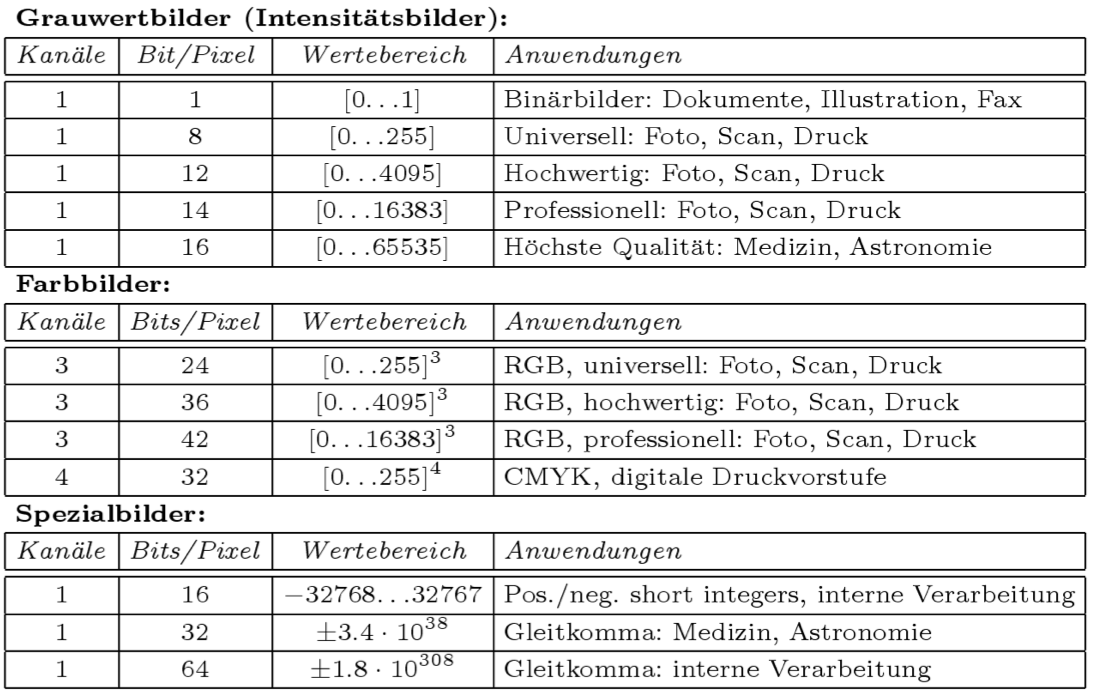
\includegraphics[scale=0.4]{pixel-wertebereiche.png} 
\end{center}

\subsection{Region of Interest}
\subsubsection*{Grundidee}
\begin{itemize}
	\item nicht immer interessieren alle Teile eines Bild gleichermassen
	\item der oder die Bildbereiche, welche von Interesse sind, werden als ROIs bezeichnet
\end{itemize}
\subsubsection*{Bildformate mit ROI-Unterstützung}
\begin{itemize}
	\item JPEG 2000 (ROIs werden weniger stark komprimiert)
	\item PGF (nur ROI wird dekomprimiert)
\end{itemize}
\subsubsection*{Bestimmung von ROIs}
\begin{itemize}
	\item manuell (Benutzerin wählt den ROI selber aus)
	\item automatisch
		\begin{itemize}
			\item Regionen mit Pixel einer bestimmten Intensität/Farbe
			\item Regionen mit erhöhter Dichte
			\item Regionen mit bestimmten Mustern (Mustererkennung)
			\item Regionen die visuell hervorragen (Saliency Detection)
		\end{itemize}
\end{itemize}

\pagebreak
\section{Bildspeicherung}

\subsection{Bildformate}
\subsubsection*{ohne Kompression}
\begin{itemize}
	\item PNM: Portable Bitmap/Grayscale/Color Format
	\item RAS: Sun Raster Format
	\item BMP: Windows Bitmap
\end{itemize}
\subsubsection*{mit verlustloser Kompression}
\begin{itemize}
	\item GIF: Graphics Interchange Format
	\item PNG: Portable Network Graphics
	\item TIFF: Tagged Image File Format
\end{itemize}
\subsubsection*{nur mit verlustloser Kompression}
\begin{itemize}
	\item JFIF: JPEG File Interchange Format
	\item EXIF: Exchangeable Image File Format (Variante von JFIF)
\end{itemize}
\subsubsection*{mit verlustloser/verlustbehafteter Kompression}
\begin{itemize}
	\item JPEG-2000
	\item PGF: Progressive Graphics File
\end{itemize}

\subsection{PGM-Beispiel}
\begin{center}
	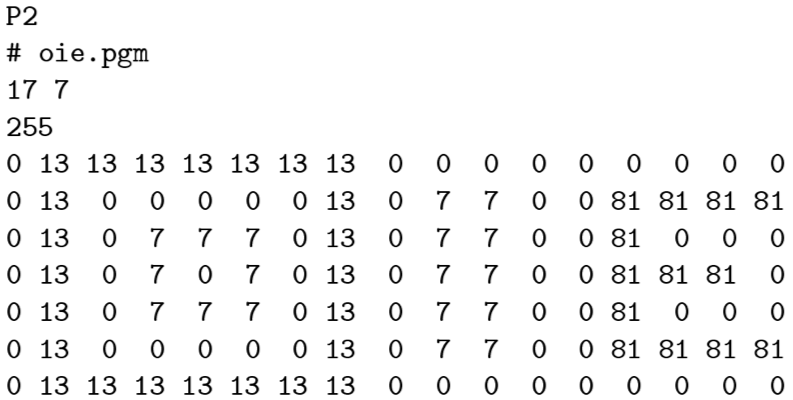
\includegraphics[scale=0.2]{pgm.png}
\end{center}

\subsection{TIFF-Struktur}
\begin{center}
	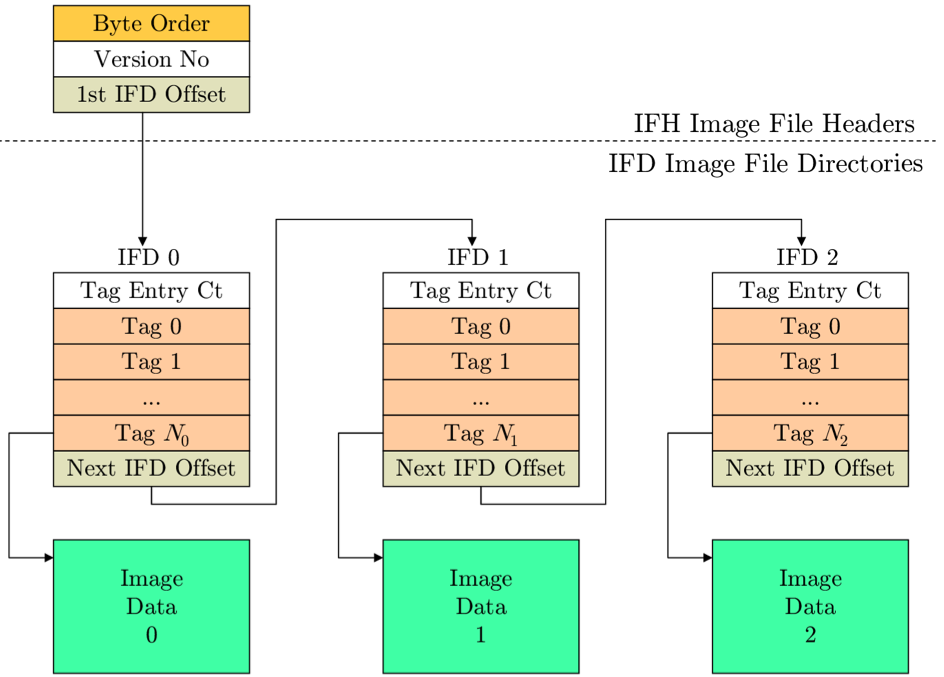
\includegraphics[scale=0.2]{tiff.png}
\end{center}

\subsection{JPEG-Prozesskette}
\begin{center}
	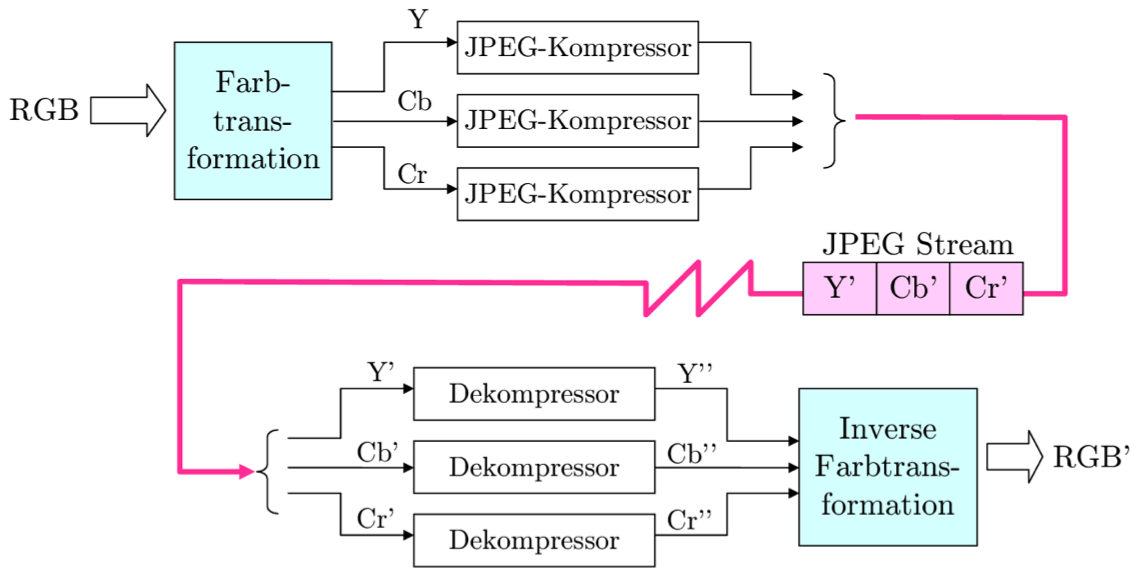
\includegraphics[scale=0.2]{jpeg.png}
\end{center}

\subsection{Bildkompression}
Das Ziel ist ein Bild auf dem Speichermedium so zu verdichten, dass es möglichst wenig Speicher benötigt, unter der Nebenbedingung, dass die Bildqualität möglichst gut ist. \\
\begin{equation*}
	\text{Kompressionsrate } r = \frac{mem_{orig}}{mem_{comp}}
\end{equation*}
\subsubsection*{verlustlos (Codierung)}
\begin{itemize}
	\item Entropiecodierung (Huffman, arithmetisch usw.)
	\item Präcodierung (RLE, LZ usw.)
\end{itemize}
\subsubsection*{verlustbehaftet (Datenreduktion)}
\begin{itemize}
	\item Farbreduktion (skalare Quantisierung / Vektorquantisierung)
	\item Transformation (Fourier / Wavelet) und Quantisierung der Koeffizienten
\end{itemize}

\subsection{Codierung}
\begin{equation*}
	\text{Codierungsredundanz } \Delta R_{cod} = S - H
\end{equation*} 
\begin{tabular}{l l}
	$N_A$ & Anzahl Symbole im Signal \\
	$N_B$ & gesamte Datenmenge des Signals in Bit \\
	$S=N_B / N_A$ & mittlere Anzahl Bits pro Symbol \\
	$K$ & Anzahl verschiedener Symbole \\
	$p_i$ & Symbol-Wahrscheinlichkeit \\
	$H=-\sum_{i=1}^K p_i*ld(p_i)$ & Entropie (mittlerer Symbolinformationsgehalt) \\
	$H_{tot} = n * H$ & Totaler Informationsgehalt bei $n$ Symbolen\\
\end{tabular}

\subsubsection{mittlere Codelänge einer Symbolfolge}
\begin{itemize}
	\item Alphabet $\{s_1, s_2, \dots s_K \}$
	\item mit $p_i$ = Auftretenswahrscheinlichkeit des Symbols $s_i$
\end{itemize}
\begin{equation*}
	l = \sum_{i=1}^K p_i * ||c_i|| \text{ [Bit/Symbol]}
\end{equation*}
\begin{equation*}
	\text{Untere Schranke } H \leq l \leq H+1 \text{ Obere Schranke}
\end{equation*}

\subsubsection{Huffman-Code}
\begin{enumerate}
	\item Betrachte alle Symbole als Blätter eines Codebaums und trage ihre Wahrscheinlichkeiten ein.
	\item Fasse die beiden geringsten Wahrscheinlichkeiten zu einem Knoten zusammen und weise ihre Summe dem Knoten zu.
	\item Beschrifte die neuen Äste mit 0 und 1.
	\item Fahre bei Schritt 2 fort, so lange die Wurzel mit Wahrscheinlichkeit p = 1 noch nicht erreicht worden ist.
\end{enumerate}
\begin{center}
	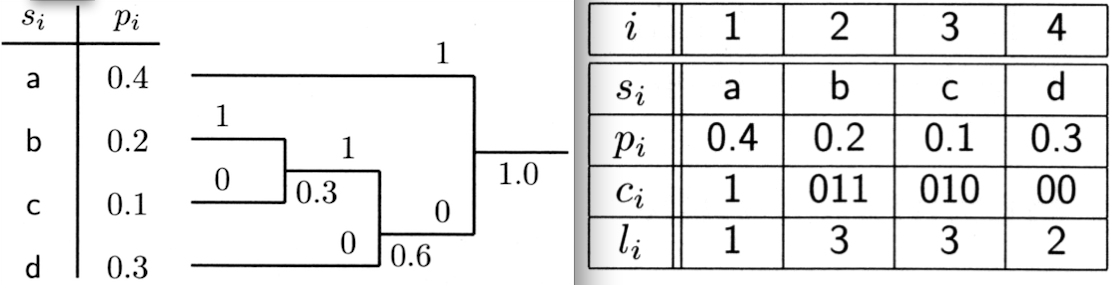
\includegraphics[scale=0.2]{huffman-code.png}
\end{center}

\subsection{Unterabtastung}
\begin{center}
	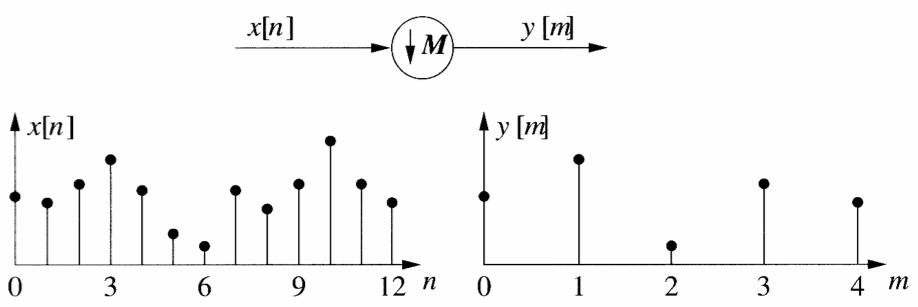
\includegraphics[scale=0.3]{unterabtastung.png}
\end{center}

\subsection{quantisierung}
\begin{center}
	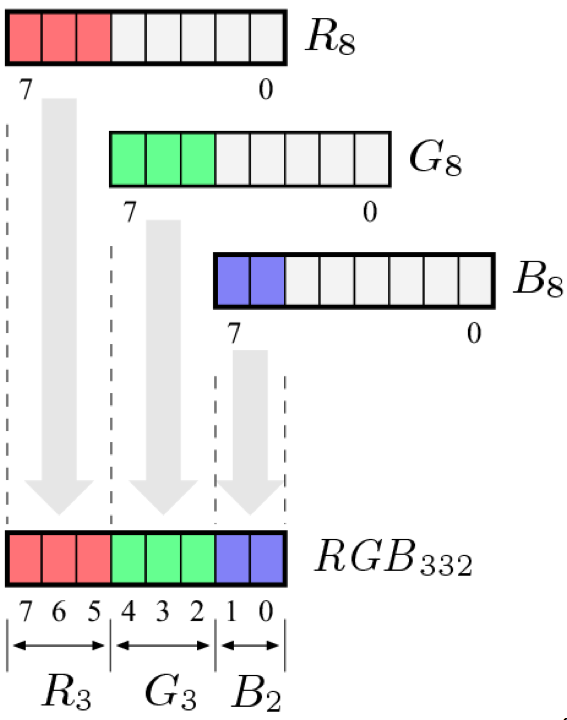
\includegraphics[scale=0.3]{quantisierung.png}
\end{center}

\pagebreak
\section{Punktoperationen}

\subsection{Definition}
\subsubsection{homogen}
\begin{equation*}
	I'(u,v) \leftarrow f(I(u,v))
\end{equation*}
Typische Beispiele:
\begin{itemize}
	\item Änderungen von Kontrast und Helligkeit
	\item Invertieren von Bildern
	\item Quantisieren der Helligkeit (Poster-Effekt)
	\item Schwellwertbildung
	\item Gammakorrektur
	\item Farbtransformation
\end{itemize}
\subsubsection{nicht homogen}
\begin{equation*}
	I'(u,v) \leftarrow g(I(u,v), u, v)
\end{equation*}
Typisches Beispiel:
\begin{itemize}
	\item selektive Kontrast - oder Helligkeitsanpassung
\end{itemize}

\subsection{Kontrast und Helligkeit}
Erhöhung des Kontrasts um 50\%:
\begin{equation*}
	I'(u,v) \leftarrow f(I(u,v)) * 1.5
\end{equation*}
Anheben der Helligkeit um 10 Stufen:
\begin{equation*}
	I'(u,v) \leftarrow f(I(u,v)) + 10
\end{equation*}

\subsection{Automatische Kontrastanpassung}
\begin{equation*}
	I'(u,v) \leftarrow \begin{cases}
  p_{min},  & \text{für } I(u,v) \leq q_{low}\\
  p_{min} + (I(u,v) - q_{low}) * \frac{p_{max}-p_{min}}{q_{high}-q_{low}},  & \text{für } q_{low} < I(u,v) < q_{high}\\
  p_{max}, & \text{für } I(u,v) \geq q_{high}\\
\end{cases}
\end{equation*}
\begin{center}
	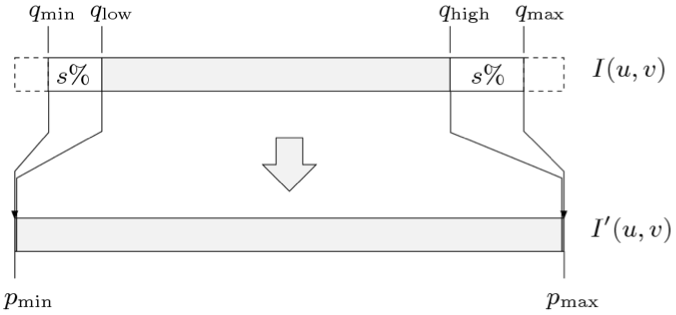
\includegraphics[scale=0.3]{kontrastanpassung.png}
\end{center}

\subsection{Schwellwertoperation}
Thresholding
\begin{itemize}
	\item Reduktion auf zwei Intensitätswerte $\rightarrow$ Binarisierung
	\item Spezialfall der Quantisierung (Graustufenreduktion)
\end{itemize}
\begin{equation*}
	I'(u,v) \leftarrow f_{th}(I(u,v)\begin{cases}
  p_0,  & \text{für } I(u,v) < p_{th}\\
  p_1, & \text{für } I(u,v) \geq p_{th}\\
\end{cases}
\end{equation*}
\begin{center}
	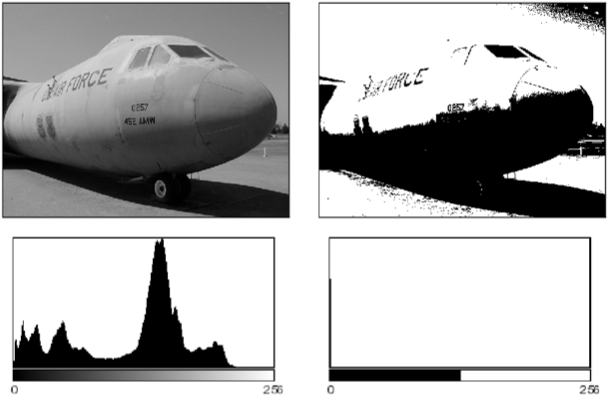
\includegraphics[scale=0.3]{schwellwertoperation.png}
\end{center}

\subsection{Histogrammausgleich}
\begin{center}
	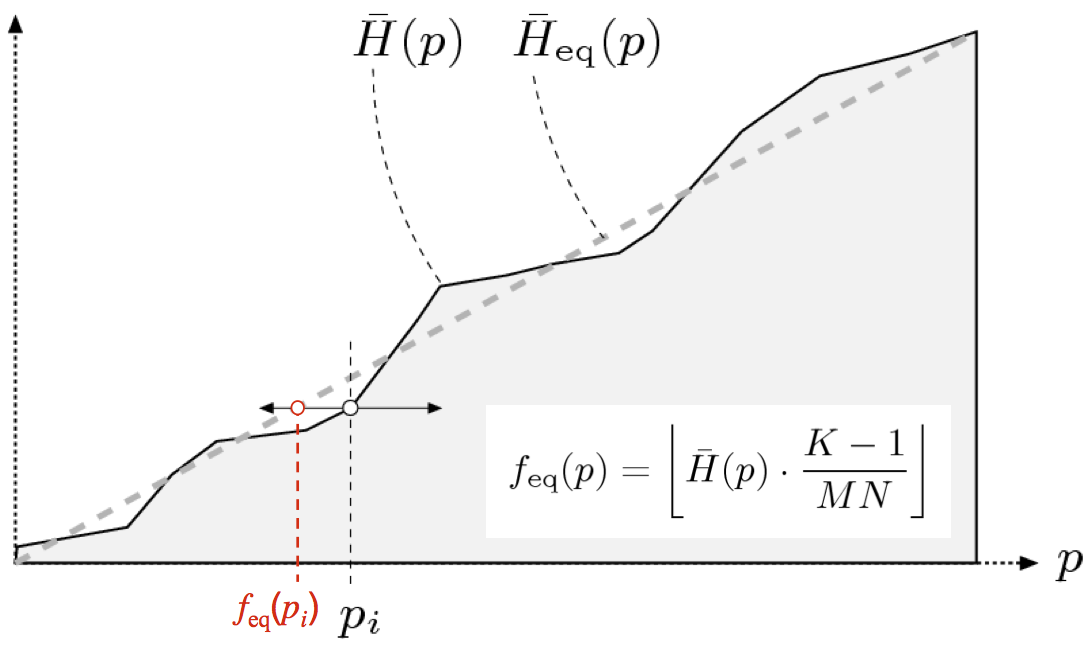
\includegraphics[scale=0.2]{histogrammausgleich.png}
\end{center}

\subsection{Gammakorrektur}
\subsubsection*{einfache Gammakorrektur}
\begin{equation*}
	q = GC(p, \gamma) = \left( \frac{p}{p_{max}}\right)^\gamma * p_{max}
\end{equation*}
\subsubsection*{Probleme}
\begin{itemize}
	\item Anstieg der Gammafunktion in der Nähe des Nullpunktes
	\item starke Rauschanfälligkeit wegen der extrem hohen Verstärkung
\end{itemize}
\subsubsection*{Modifizierte Gammafunktion}
\begin{equation*}
	s = \frac{\gamma}{x_0(\gamma-1)+x_0^{1-\gamma}} \hspace{2cm} d = \frac{1}{x_0^\gamma(\gamma-1)+1}-1
\end{equation*}
Gammakorrektur:
\begin{equation*}
	f_{(\gamma, x_0)}(x) = \begin{cases}
		s * x, & \text{für } 0 \leq x \leq x_0 \\
		(1+d) * x^\gamma - d, & \text{für } x_0 < x \leq 1
	\end{cases}
\end{equation*}
Inverse Gammakorrektur:
\begin{align*}
	f_{(\gamma, x_0)}(y) = \begin{cases}
		\frac{y}{s}, & \text{für } y \leq s \cdot x_0 \\
		\left( \frac{y+d}{1+d} \right)^\frac{1}{\gamma}, & \text{für } y > s \cdot x_0
	\end{cases}
\end{align*}


\subsection{Bildqualität}
\begin{itemize}
	\item technische Bildqualität ist ein Mass für die Abweichung zwischen Original (o) und Kopie (k)
	\item eine subjektive Qualitätsmessung eines Betrachters kännte anders ausfallen
\end{itemize}
\subsubsection*{root mean squared error}
Bildkanal mit n Pixeln:
\begin{equation*}
	RMSE = \sqrt{\frac{\sum_{i=1}^n (o[i]-k[i])^2}{n}}
\end{equation*}
\subsubsection*{peak signal-to-noise ratio in dB}
Bildkanal mit maximaler Intensität 255:
\begin{equation*}
	PSNR = 20 * log_{10} \left( \frac{255}{RMSE} \right)
\end{equation*}

\pagebreak
\section{Farben}

\subsection{Farbsysteme}
\subsubsection{lineare Farbsysteme}
\textbf{RGB:}
\begin{itemize}
	\item Rot, Grün, Blau
	\item additive Farbmischung
\end{itemize}
\textbf{CMY:}
\begin{itemize}
	\item Cyan (Türkis), Magenta (Purpur), Yellow (Gelb)
	\item subtraktive Farbmischung
\end{itemize}
\textbf{CMY:}
\begin{itemize}
	\item Cyan (Türkis), Magenta (Purpur), Yellow (Gelb)
	\item subtraktive Farbmischung
\end{itemize}
\textbf{YUV, YIQ und $YC_bC_r$:}
\begin{itemize}
	\item Fernseh-Komponentenfarbräume
\end{itemize}
\textbf{CIEXYZ:}
\begin{itemize}
	\item CIE Standard-Farbraum
\end{itemize}
\subsubsection{niht lineare Farbsysteme}
\textbf{CMYK:}
\begin{itemize}
	\item Farbmischung für den 4-Farbendruck: CMY und Schwarz (K)
\end{itemize}
\textbf{HSV/HSB/HSI/HLS:}
\begin{itemize}
	\item Hue (Farbton), Saturation (Sättigung), Value/Brightness/Intensity/Luminance (Helligkeit)
\end{itemize}
\textbf{CIExy:}
\begin{itemize}
	\item Koordinatensystem des CIE-Farbdiagramms
	\item einfache Umrechnung zwischen CIEXYZ und CIExy
	\item nicht intuitiv zu verstehen
\end{itemize}
\textbf{CIE L*a*b*:}
\begin{itemize}
	\item intuitiv verständlich
	\item möglichst linear gegenüber dem menschlichen Sehen
\end{itemize}
\textbf{sRGB:}
\begin{itemize}
	\item Standard RGB (präzise definiert, basierend auf CIE xy)
	\item relativ kleines Gamut (für digitale Anwendungen genügend)
\end{itemize}

\subsection{Farbräume}
\subsubsection{RGB}
\begin{center}
	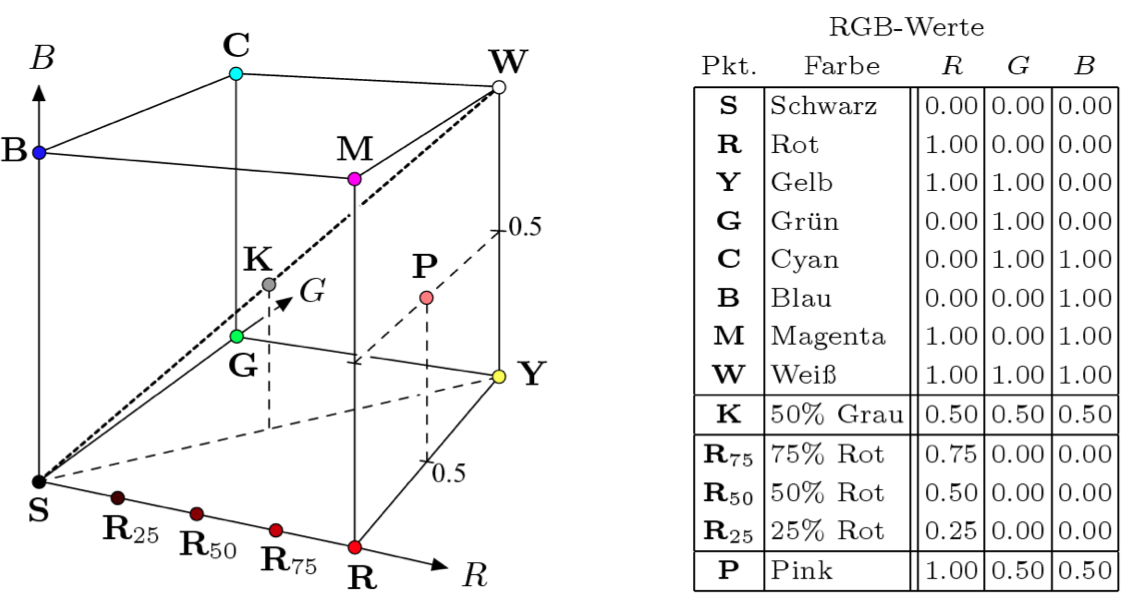
\includegraphics[scale=0.2]{rgb.png}
\end{center}
\subsubsection{HSV und HLS}
\begin{center}
	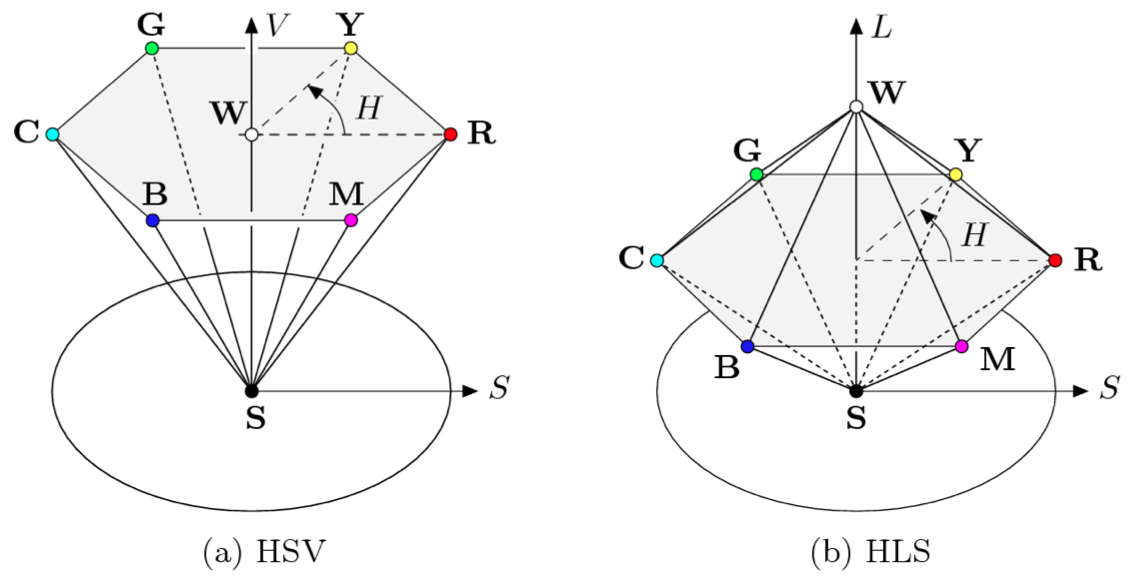
\includegraphics[scale=0.2]{hsv-und-hls.png}
\end{center}
\subsubsection{CIExyz}
\begin{center}
	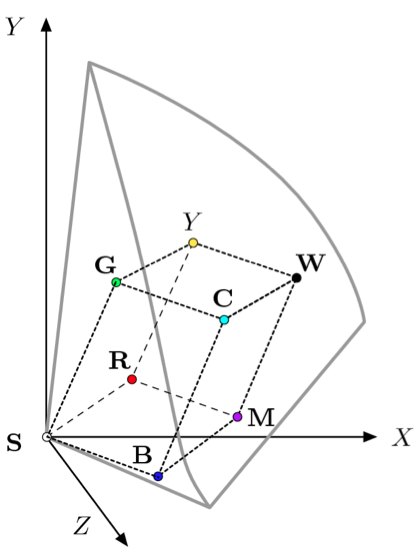
\includegraphics[scale=0.2]{cie_xyz.png}
\end{center}
\subsubsection{CIExy}
\begin{center}
	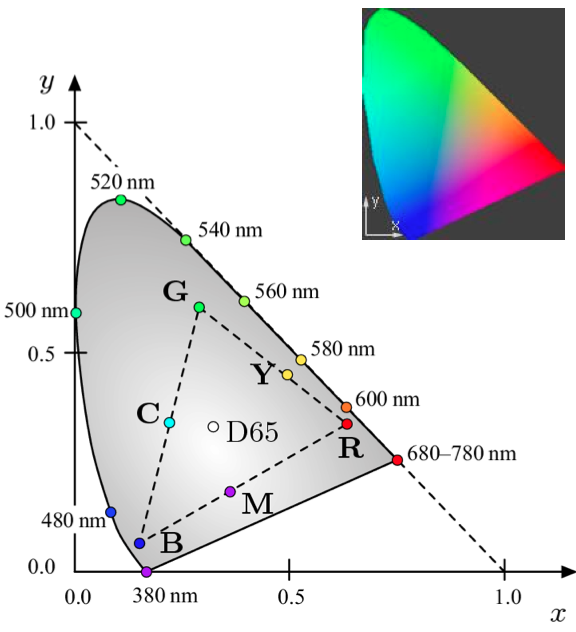
\includegraphics[scale=0.2]{cie_xy.png}
\end{center}

\subsection{Umwandlungen}
\subsubsection{CMY und CMYK}
\textbf{RGB $\rightarrow$ CMY:}
\begin{align*}
	C &= 1-R \\
	M &= 1-G \\
	Y &= 1-B
\end{align*}
\textbf{CMY $\rightarrow$ CMYK:}
\begin{align*}
	C' &= C-K \\
	M' &= M-K \\
	Y' &= Y-K \\
	K' &= K
\end{align*}
\subsubsection{CIExy}
\textbf{XYZ $\rightarrow$ xy:}
\begin{equation*}
	x= \frac{X}{X+Y+Z} \hspace{2cm} y= \frac{Y}{X+Y+Z}
\end{equation*}
\textbf{xy $\rightarrow$ XYZ:}
\begin{equation*}
	X=\frac{x}{y}\hspace{2cm} Y=1 \hspace{2cm} Z = \frac{z}{y} = \frac{1-x-y}{y}
\end{equation*}
\subsubsection{Transformation sRGB $\rightarrow$ XYZ}
Nichtlineare sRGB-Komponenten: 
\begin{equation*}
	R = f_2(R') \hspace{2cm} G = f_2(G') \hspace{2cm} B = f_2(B')
\end{equation*}
Inverse modifzierte Gammakorrektur \\
\\
Lineare Transformation von RGB nach CIE XYZ:
\begin{equation*}
	\begin{pmatrix} X \\ Y \\ Z \end{pmatrix} = \begin{pmatrix} 0.4124 & 0.3576 & 0.1805 \\0.2126 & 0.7152 & 0.0722 \\ 0.0193 & 0.1192 & 0.9505\end{pmatrix} \cdot \begin{pmatrix} R \\ G \\ B \end{pmatrix}
\end{equation*}
Rücktransformation:
\begin{equation*}
	\begin{pmatrix} R \\ G \\ B \end{pmatrix}= \begin{pmatrix} 3.2406 & -1.5372 & -0.4986 \\ -0.9689 & 1.8758 & 0.0415 \\ 0.0557 & -0.2040 & 1.0570 \end{pmatrix} \cdot \begin{pmatrix} X \\ Y \\ Z \end{pmatrix} 
\end{equation*}
\subsection{Weisspunkte}
\begin{description}
	\item[D50] \hfill
		\begin{itemize}
			\item Farbtemperatur von 5000 Kelvin
			\item ähnlich dem direkten Sonnenlicht
			\item Referenzbeleuchtung für die Betrachtung von reflektierenden Bildern wie z.B. von Druckern
		\end{itemize}
	\item[D65] \hfill
		\begin{itemize}
			\item Farbtemperatur von 6500 Kelvin
			\item durchschnittliche indirekte Tageslichtbeleuchtung
			\item Normweisslicht für emittierende Wiedergabegeräte z.B. von Bildschirme
		\end{itemize}
\end{description}
\subsubsection*{Chromatische Adaptierung:}
\begin{equation*}
	\begin{pmatrix} X_{65} \\ Y_{65} \\ Z_{65} \end{pmatrix} = 
	M_{65|50} \cdot \begin{pmatrix} X_{50} \\ Y_{50} \\ Z_{50} \end{pmatrix} = 
	\begin{pmatrix} 
	0.955556 & -0.023049 & 0.063197 \\
	 -0.028302 & 1.009944 & 0.021018 \\
	  0.012305 & -0.020494 & 1.330084
	  \end{pmatrix} \cdot \begin{pmatrix} X_{50} \\ Y_{50} \\ Z_{50} \end{pmatrix} 
\end{equation*}

\begin{equation*}
	\begin{pmatrix} X_{50} \\ Y_{50} \\ Z_{50} \end{pmatrix} = 
	M_{50|65} \cdot \begin{pmatrix} X_{65} \\ Y_{65} \\ Z_{65} \end{pmatrix} =
	 \begin{pmatrix} 
	1.047840 & 0.0228961 & -0.0501482\\ 
	0.0295561 & 0.990482 & -0.0170559 \\
	 -0.00923843 & 0.0150496 & 0.752033
	 \end{pmatrix} \cdot \begin{pmatrix} X_{65} \\ Y_{65} \\ Z_{65} \end{pmatrix} 
\end{equation*}

\pagebreak
\section{Filter}

\subsection{Anwendung}
\begin{center}
	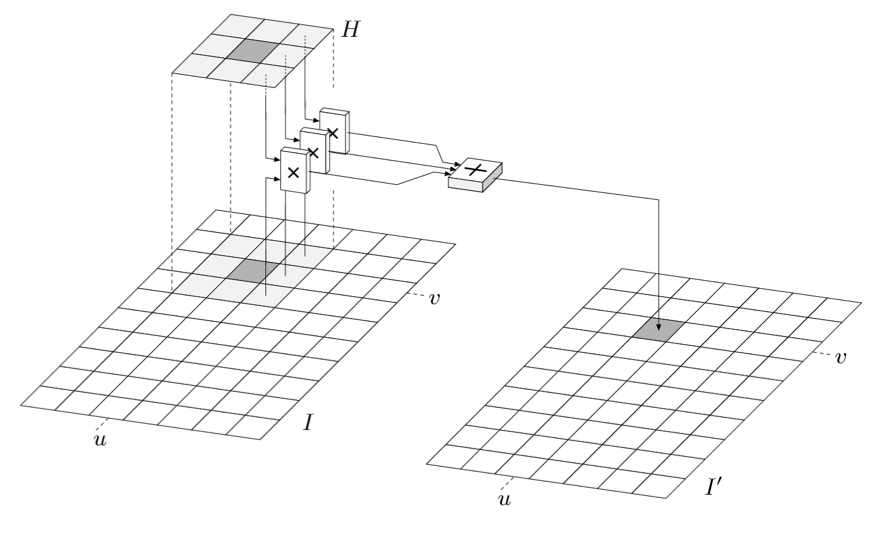
\includegraphics[scale=0.3]{filter-anwendung.png}
\end{center}
\begin{equation*}
	I'(u,v) \leftarrow \sum_{(i,j)\in \RN} I(u+ i, v+j) * H(i,j)
\end{equation*}

\subsection{Gauss-Filter}
diskrete, zweidimensionale Gauss-Funktion:
\begin{equation*}
	G_\sigma(r) = e^{-\frac{r^2}{2\sigma^2}} \hspace{2cm} G_\sigma(x, y) = e^{-\frac{x^2+y^2}{2\sigma^2}}
\end{equation*}
Glättungsfilter (Tiefpassfilter):
\begin{itemize}
	\item weil alle Filterkoeffizienten positiv sind
	\item annähernd isotrop ab Filtergrössen von 5 x 5 (nach allen Richtungen hin gleichförmig arbeiten)
	\item gutmütiges Frequenzverhalten (stetig, differenzierbar)
\end{itemize}

\subsection{Laplace-Filter}
Interpretation als Differenz von zwei Summen:
\begin{equation*}
	I'(u,v) = \sum_{(i,j)\in \RN^+} I(u+i,v+j)*|H(i,j)| - \sum_{(i,j)\in \RN^-} I(u+i,v+j)*|H(i,j)|
\end{equation*}
$\RN^+/\RN^-$ Teil der Filterregion mit positiven/negativen Koeffizienten \\
\\
Verstärken von Kanten und Konturen:
\begin{itemize}
	\item örtliche Intensitätsunterschiede werden verstärkt
	\item richtungsunabhängige Detektion von Kanten
	\item Hochpassfilter
\end{itemize}

\subsection{Faltung}
\subsubsection{diskrete Faltung}
\begin{align*}
	I'(u,v) &= \sum_{i=-\infty}^\infty \sum_{j=-\infty}^\infty I(u-i,v-j) \cdot H(i,j) \\
	I' &= I*H \\
	I'(u,v) &= \sum_{(i,j) \in \RN} I(u-i,v-j) \cdot H(i,j) \\
	 &= \sum_{(i,j) \in \RN} I(u+i,v+j) \cdot H(-i,-j) \\
\end{align*}
\subsubsection{Eigenschaften der Faltung}
\begin{align*}
 \text{Kommutativität:} \\
	I*H &= H * I \\
	\text{Linearität:} \\
	(a \cdot I) * H &= I * (a \cdot H) = a \cdot (I*H) \\
	(I_1 + I_2) * H &= (I_1 * H) + (I_2 * H) \\
	\text{Assoziativität:} \\
	A * (B * C) &= (A * B ) * C
\end{align*}

\subsection{Separierbarkeit}
\begin{equation*}
	I' \leftarrow (I*H_x)*Hy = I * \underbrace{(H_x*H_y)}_{H_{xy}}
\end{equation*}
\begin{center}
	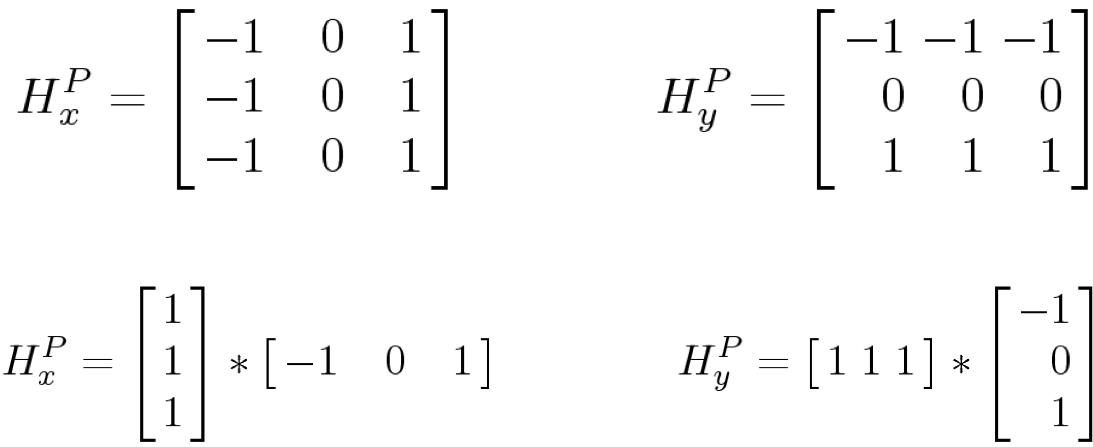
\includegraphics[scale=0.2]{separierbarkeit.png}
\end{center}

\pagebreak
\section{Morphologie}

\subsection{Schrumpfen und Wachsen}
\begin{center}
	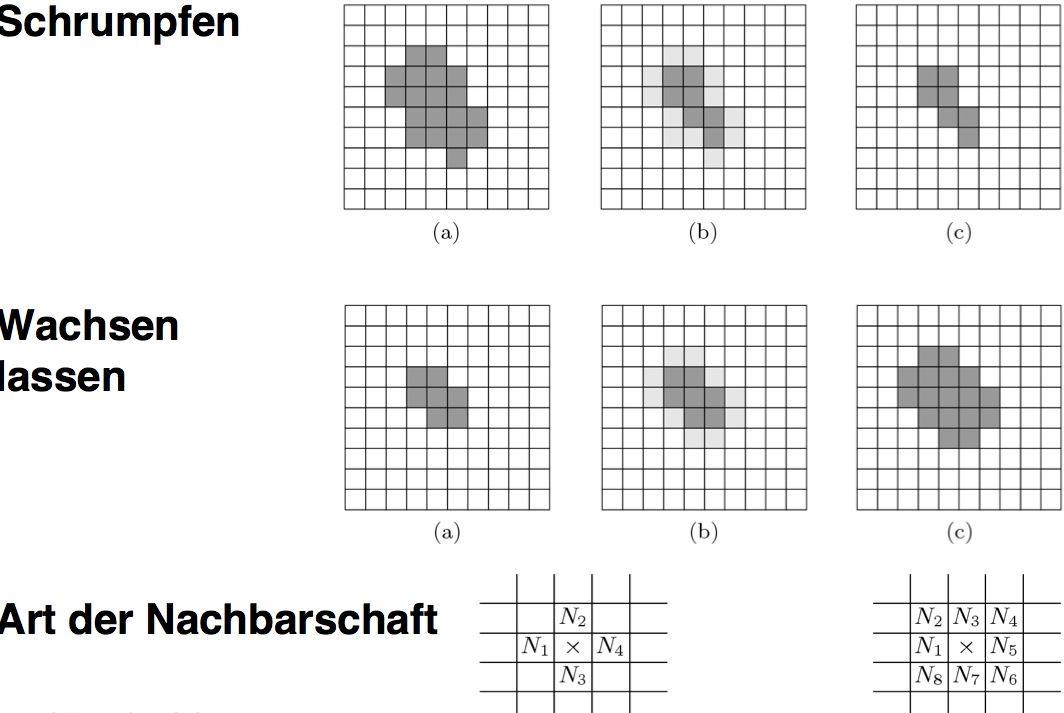
\includegraphics[scale=0.25]{schrumpfen-und-wachsen.png}
\end{center}

\subsection{Grundoperationen}
\textbf{Strukturelement}: binäre Matrix mit Hot-Spot als Ursprung des Koordinatensystems (analog zu einem Filter mit binären Koeffizienten) \\
\\
Strukturelement als Punktmenge:
\begin{equation*}
	P_H=\{(i,j)|H(i,j) ) 1 \}
\end{equation*}
Bild als Punktmenge:
\begin{equation*}
	P_I=\{(u,v)|I(u,v) ) 1 \}
\end{equation*}
Erosion (Schrumpfen):
\begin{equation*}
	I \ominus H=\{ (x,y) | (x + i, y + j) \in P_i, \forall (i,j) \in PH \}
\end{equation*}
\begin{center}
	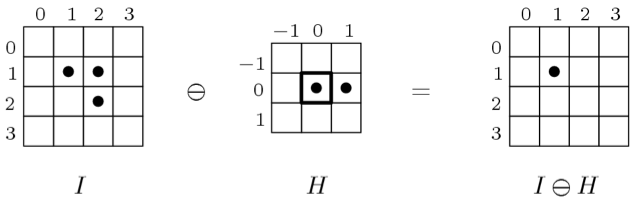
\includegraphics[scale=0.25]{erosion.png}
\end{center}
Dilation (Wachsen lassen):
\begin{equation*}
	I \oplus H=\{ (x,y) = (u + i, v + j) | (u, v) \in P_i, \forall (i,j) \in PH \}
\end{equation*}
\begin{center}
	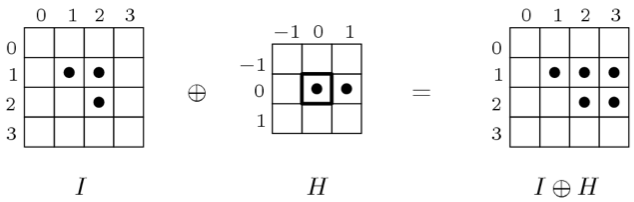
\includegraphics[scale=0.25]{dilation.png}
\end{center}

\subsection{Zusammengesetzte Operationen}
\subsubsection*{Opening}
zuerst schrumpfen, dann wachsen lassen:
\begin{equation*}
	I \circ H = (I \ominus H) \oplus H
\end{equation*}
\begin{itemize}
	\item sehr kleine Vordergrundstrukturen werden eliminiert
	\item glättet Kanten von grösseren Elementen
	\item Elemente mit kleinem Berührungspunkt werden getrennt
\end{itemize}
\subsubsection*{Closing}
zuerst wachsen lassen, dann schrumpfen:
\begin{equation*}
	I \bullet H = (I \oplus H) \ominus H
\end{equation*}
\begin{itemize}
	\item füllt kleine Löcher
	\item glättet Kanten von grösseren Elementen
	\item Elemente mit kleinem Berührungspunkt werden stärker verbunden
\end{itemize}

\subsection{Grauwert-Morphologie}
\subsubsection*{Grauwert-Dilation}
\begin{equation*}
	(I \oplus H)(u, v) = \max_{(i,j) \in H} \{ I(u+i,v+j) + H(i,j) \}
\end{equation*}
\begin{center}
	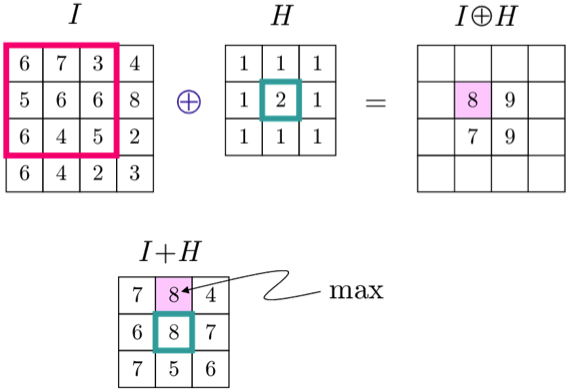
\includegraphics[scale=0.25]{grauwert-dilation.png}
\end{center}
\subsubsection*{Grauwert-Erosion}
\begin{equation*}
	(I \ominus H)(u, v) = \min_{(i,j) \in H} \{ I(u+i,v+j) - H(i,j) \}
\end{equation*}
\begin{center}
	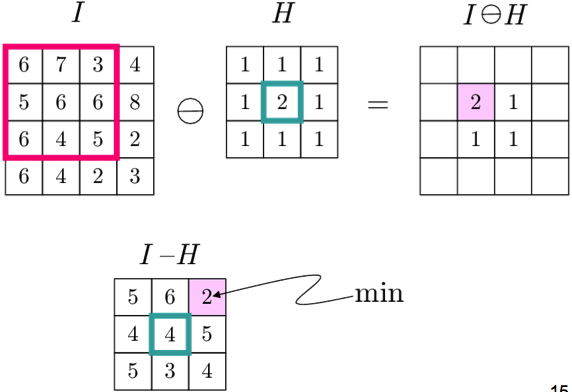
\includegraphics[scale=0.25]{grauwert-erosion.png}
\end{center}

\pagebreak
\section{Binärbildanalyse}

\subsection{Prozesskette}
\begin{center}
	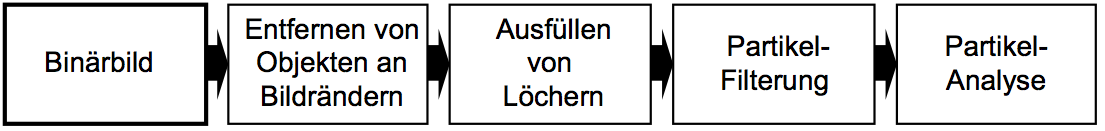
\includegraphics[scale=0.25]{partikelprozesskette.png}
\end{center}

\subsection{Flood filling}
\begin{center}
	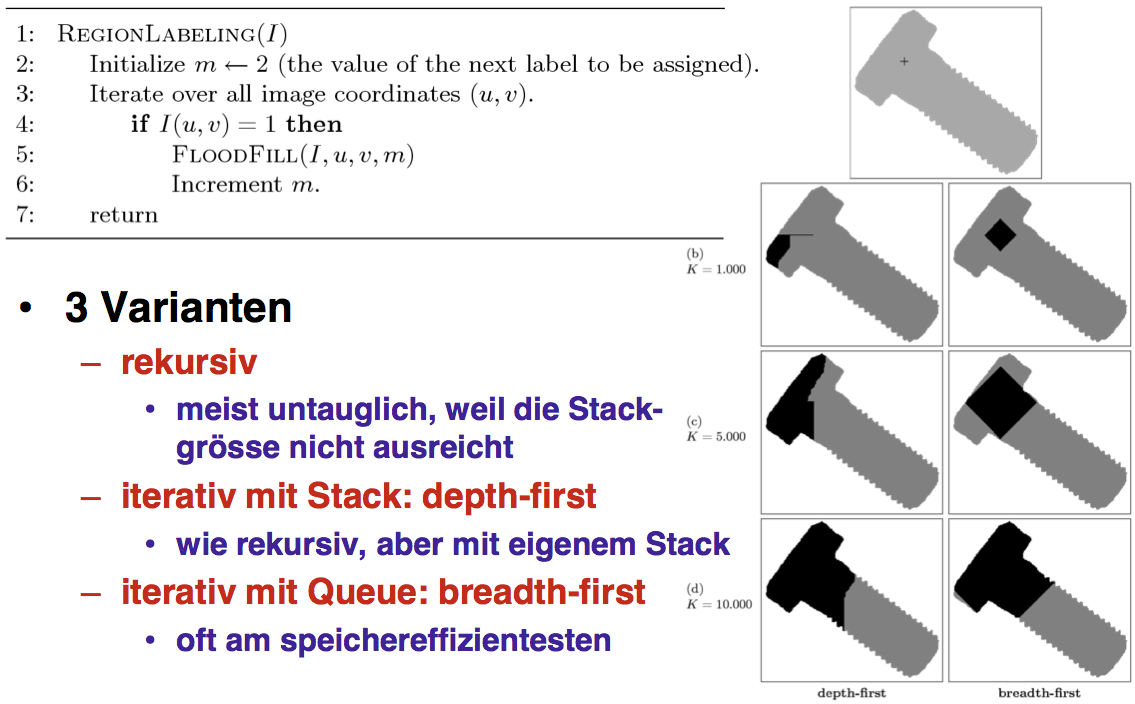
\includegraphics[scale=0.25]{flood_filling.png}
\end{center}

\subsection{Rekursives Flood Filling}
\begin{center}
	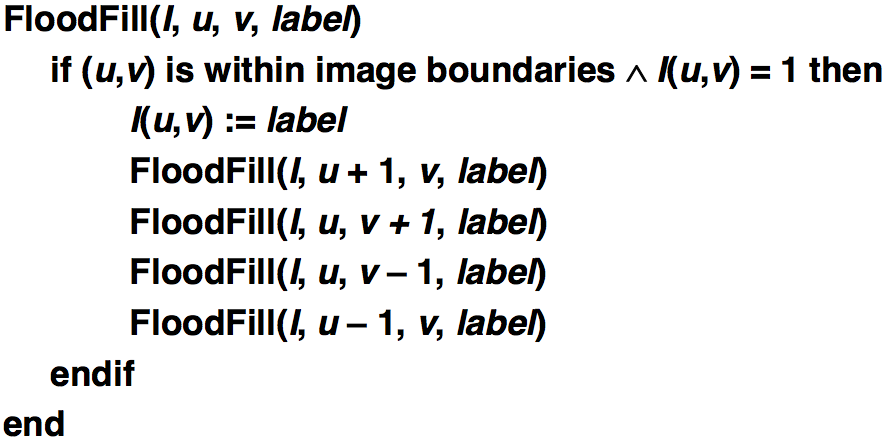
\includegraphics[scale=0.15]{rec_flood_filling.png}
\end{center}

\subsection{Hough-Transformation}
Die Grundidee ist, dass wir durch alle Kantenpixen in einem binären Kantenbild gehen. Ein solches Kantenpixel entspricht einem Punkt im Bildraum. Durch einen solchen Punkt im Bildraum können undendliche viele verschiedenen Geraden im Bildraum laufen. Diese können durch eine einzige Gerade im Parameterraum repräsentiert werden. Liegen mehrere Punkte im Bildraum auf derselben Geraden im Bildraum, so schneiden sich die entsprechenden Geraden im Parameterraum in einem einzigen Punkt.
\begin{center}
	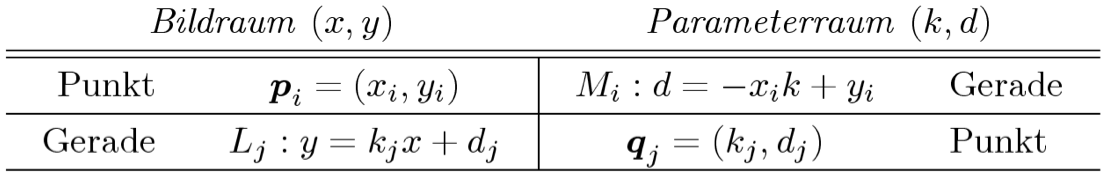
\includegraphics[scale=0.25]{ht-geraden.png} \\
	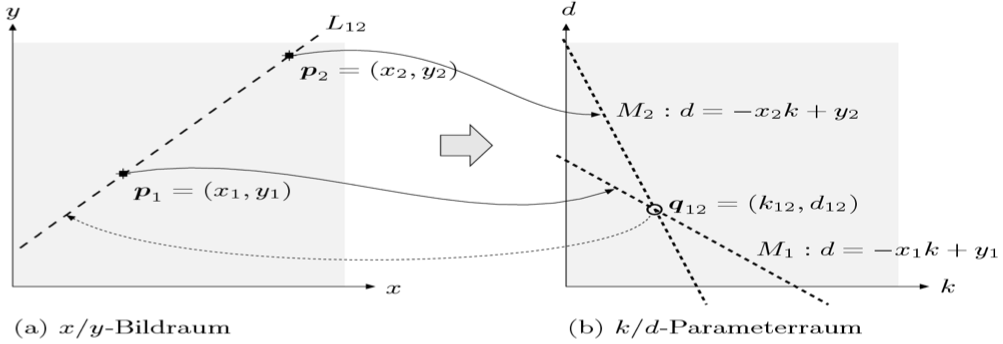
\includegraphics[scale=0.25]{ht-geraden-2.png}
\end{center}

\pagebreak
\section{Mustererkennung (Pattern Matching)}

\subsection{Definitionen}
\begin{center}
	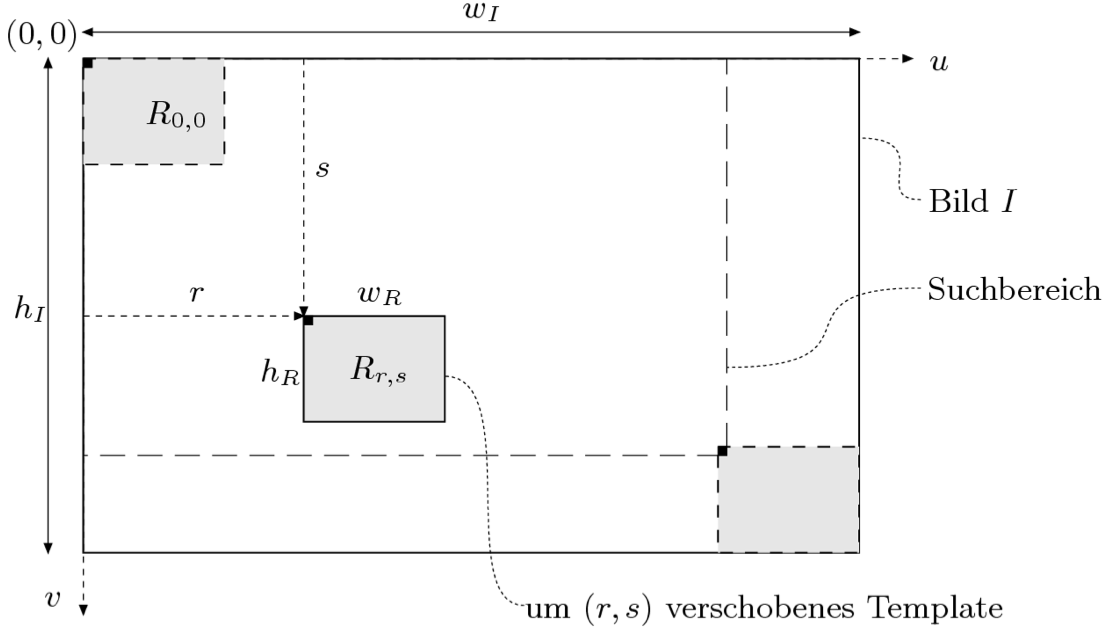
\includegraphics[scale=0.3]{pm-definitionen.png}
\end{center}

\subsection{Ähnlichkeitsmasse}
Summe der Differenzbeträge:
\begin{equation*}
	d_A(r, s) = \sum_{(i,j) \in \RN} | I(r+i,s+j) - R(i,j)|
\end{equation*}
Maximaler Differenzbetrag
\begin{equation*}
	d_M(r, s) = \max_{(i,j) \in \RN} | I(r+i,s+j) - R(i,j)|
\end{equation*}
Summe der der quadratischen Differenzbeträge (euklidische Distanz):
\begin{equation*}
	d_E(r, s) = \sqrt{\sum_{(i,j) \in \RN} \left( I(r+i,s+j) - R(i,j) \right)^2}
\end{equation*}
globale lineare Krezkorrelation:
\begin{equation*}
	( I \circledast R)(r,s) = \sum_{(i,j) \in \RN}  I(r+i,s+j) \cdot R(i,j) 
\end{equation*}

\subsection{Chamfer-Algorithmus}
\begin{center}
	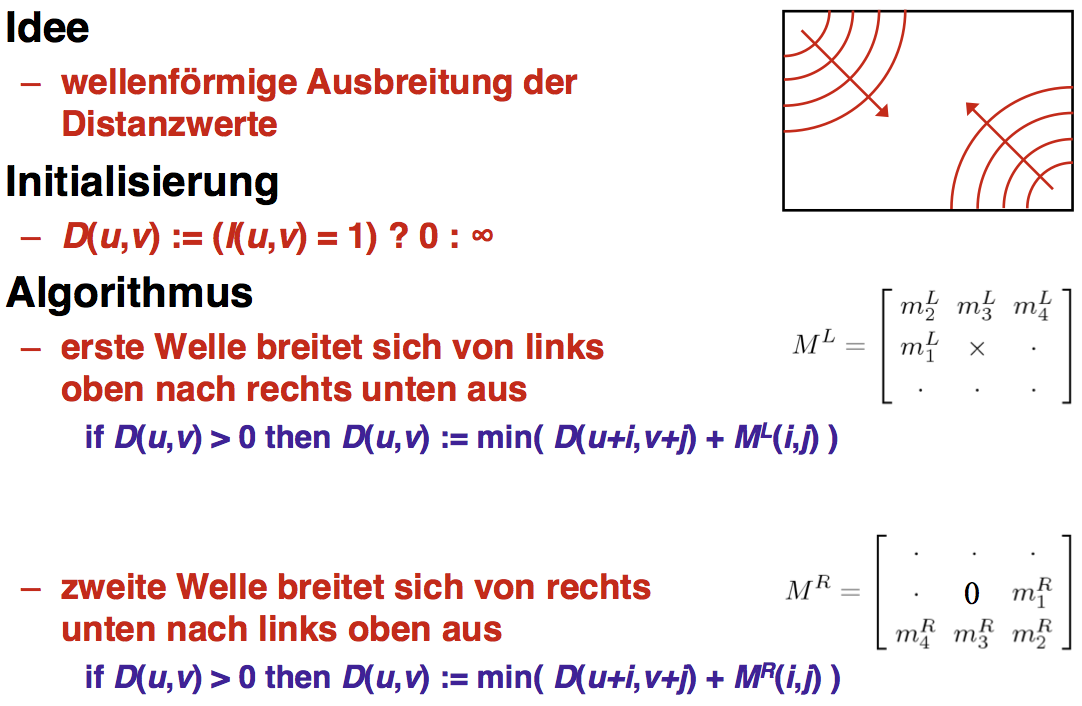
\includegraphics[scale=0.2]{chamfer-alg.png}
	\hspace{1cm}
	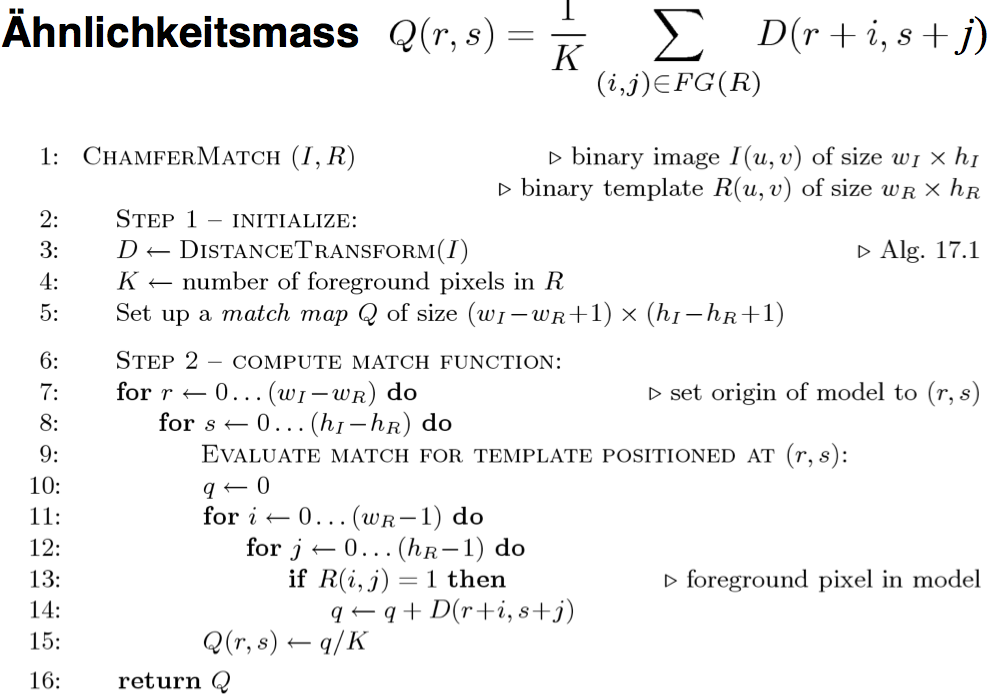
\includegraphics[scale=0.2]{chamfer-match.png}
\end{center}

\pagebreak
\section{Fourier-Transformation}

\subsection{Frequenz, Amplitude, Phase}
\begin{align*}
	\text{Beispiel} &: a \cdot sin(\omega \cdot x - \varphi) \\
	\text{Kreisfrequenz} &: \omega = 2 \cdot \pi \cdot f \\
	\text{Frequenz} &: f = \frac{1}{T} = \frac{\omega}{2 \cdot \pi} \\
	\text{Periodenlänge} &: T \\
	\text{Amplitutde} &: a \\
	\text{Phase} &: \varphi 
\end{align*}

\subsection{Fourierreihe}
Jede periodische Funktion $g(x)$ mit einer Grundfrequenz $\omega_0$ kann als unendliche Summe von harmonischen Schwingungen dargestellt werden:
\begin{equation*}
	g(x) = \sum_{k=0}^\infty \left[ A_k \cdot cos(k \cdot \omega_0 \cdot x) + B_k \cdot sin(k \cdot \omega_0 \cdot x) \right]
\end{equation*}
\textbf{Fourieranalyse:} Berechnung der Fourierkoeffizienten ($A_k$, $B_k$) aus einer gegebenen Funktion $g(x)$.

\subsection{Fourierintegral und -spektrum}
Eine nicht periodische Funktion $g(x)$ kann als Summe von unendlich vielen Sinus- und Kosinusschwingungen dargestellt werden. Das bedarf nicht nur Vielfache von der Grundfrequenz ($\rightarrow$ Fourierintegral) sondern auch unendlich viele dicht aneinander liegende Frequenzen.
\begin{equation*}
	g(x) = \int_0^\infty A_\omega \cdot cos(\omega \cdot x) + B_\omega \cdot sin(\omega \cdot x) d\omega
\end{equation*}
\textbf{Bestimmung des Fourierspektrums} (Fourierkoeefizientenfunktionen):
\begin{align*}
	A_\omega = A(\omega) &= \frac{1}{\pi} \cdot \int_{-\infty}^\infty g(x) \cdot cos(\omega \cdot x) dx \\
	B_\omega = B(\omega) &= \frac{1}{\pi} \cdot \int_{-\infty}^\infty g(x) \cdot sin(\omega \cdot x) dx \\
\end{align*}

\subsection{Fouriertransformation}
Übergang von Fourierintegral zu Fouriertransformation:
\begin{align*}
	G(\omega) &= \sqrt{\frac{\pi}{2}} \cdot \left[ A(\omega) - i \cdot B(\omega) \right] \\
	 &= \sqrt{\frac{\pi}{2}} \cdot \left[ \frac{1}{\pi} \cdot \int_{-\infty}^\infty g(x) \cdot cos(\omega \cdot x) dx - i \cdot  \frac{1}{\pi} \cdot  \int_{-\infty}^\infty g(x) \cdot sin(\omega \cdot x) dx \right] \\
	 &= \frac{1}{\sqrt{2 \pi}} \cdot \int_{-\infty}^\infty g(x) \cdot \left[ cos(\omega \cdot x) - i \cdot sin(\omega \cdot x) \right] dx
\end{align*}
\subsubsection*{Vorwärtstransformation}
\begin{equation*}
	G(\omega) = \frac{1}{\sqrt{2 \pi}} \cdot \int_{-\infty}^\infty g(x) \cdot e^{-i \omega x} dx
\end{equation*}
\subsubsection*{Rücktransformation}
\begin{equation*}
	G(\omega) = \frac{1}{\sqrt{2 \pi}} \cdot \int_{-\infty}^\infty g(x) \cdot e^{i \omega x} dx
\end{equation*}

\subsection{Fourier-Transformationspaare}
\begin{center}
	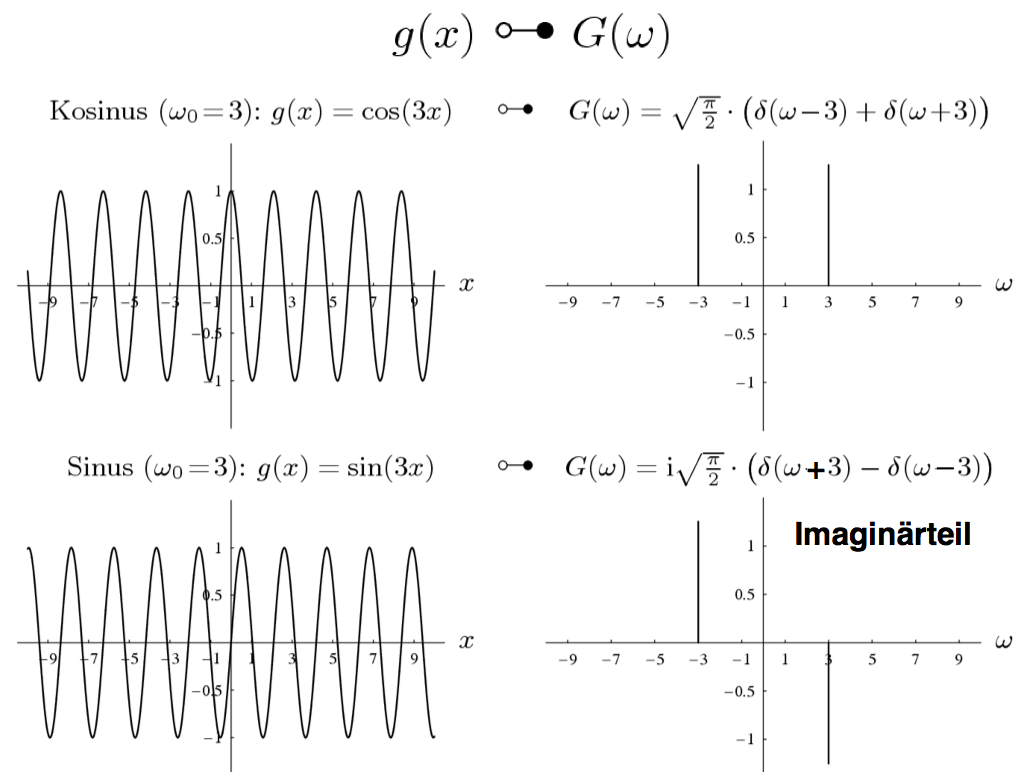
\includegraphics[scale=0.225]{ft-paar-1.png}
	\hspace{0.5cm}
	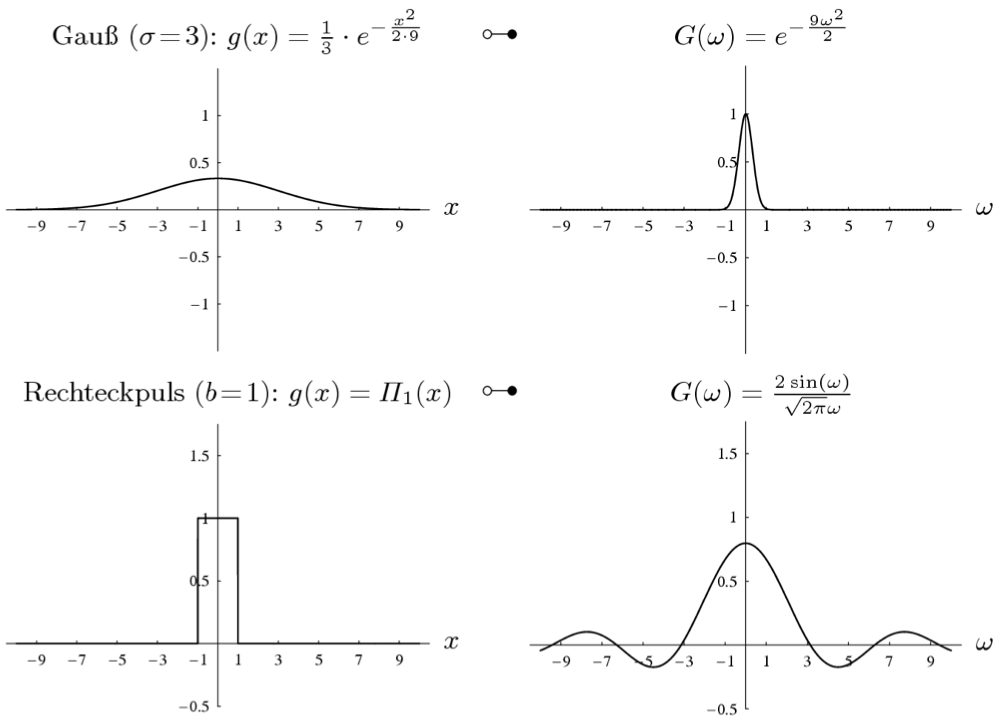
\includegraphics[scale=0.225]{ft-paar-2.png}
\end{center}
\subsection{Beispiel: Rücktransformation}
\begin{align*}
  G(\omega) &= \sqrt{\frac{\pi}{2}}(\delta(\omega-3)+\delta(\omega+3)) \\
  f(x) &= \frac{\int_{-\infty}^\infty G(\omega)e^{j\omega x}d\omega}{\sqrt{2\pi}} \\
  &= \frac{\int_{-\infty}^\infty \delta(\omega-3)e^{j\omega x}d\omega + \int_{-\infty}^\infty \delta(\omega+3)e^{j\omega x}d\omega}{2} \\
  &= \frac{e^{j3x}+e^{-j3x}}{2} \hspace*{1cm}| e^{ix} == \cos(x)+i\sin(x)\\
  &= \frac{\cos(3x)+j\sin(3x)+\cos(3x)-j\sin(3x)}{2} \\
  &= \cos(3x)
\end{align*}

\subsection{FT von diskreten Signalen}
\begin{center}
	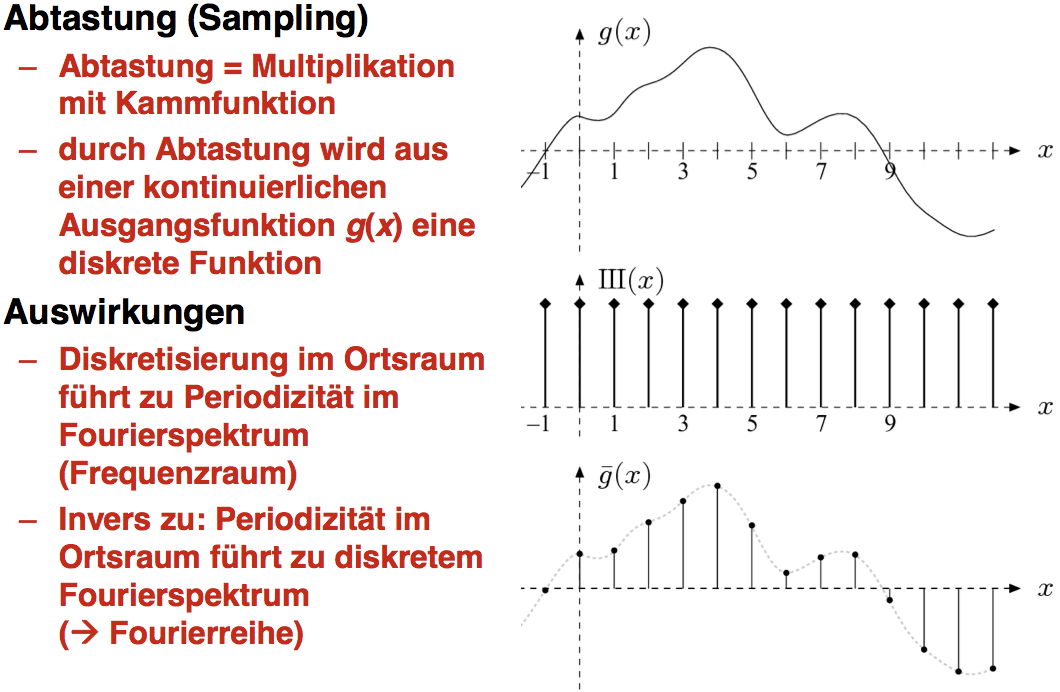
\includegraphics[scale=0.225]{ft-diskrete-signale.png}
\end{center}

\subsection{Aliasing und Abtasttheorem}
\begin{itemize}
	\item Diskretisierung im Ortsraum $\rightarrow$ Periodizität im Frequenzraum
	\item falls die sich wiederholdenden Spektralkomponenten im Frequenzraum nicht überschneiden, so ist eine verlustlose Rücktransformation möglich
	\item maximal zulässige Signalfrequenz $\omega_{max}$ ist von der Abtastfrequenz $\omega_s$ abhängig
\end{itemize}
\begin{center}
	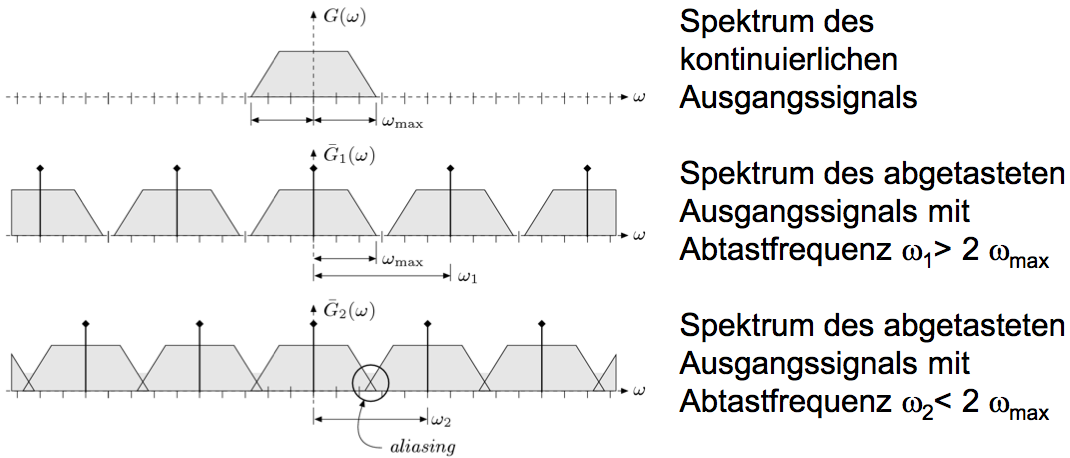
\includegraphics[scale=0.225]{ft-abtasttheorem.png}
\end{center}

\subsection{Diskrete Fouriertransformation}
\begin{figure}[h]
	\begin{floatrow}
		\capbtabbox{%
			\begin{tabular}{l l}
				Periodenlänge $t_0$: & $M$ Abtastwerte im Abstand $t_s$\\
				Frequenz $f_0$ = & $\frac{1}{M \cdot t_s}$ \\
				Abtastfrequenz $fs$ = & $\frac{1}{t_s} = M \cdot f_0$ \\
				Wellenzahl $m$: & $0 \leq m < M$ \\
				Kreisfrequenz $\omega$ & $=m \cdot \omega_0 = 2\pi \cdot m \cdot f_0$
			\end{tabular}
		}{}
		\ffigbox{}{
			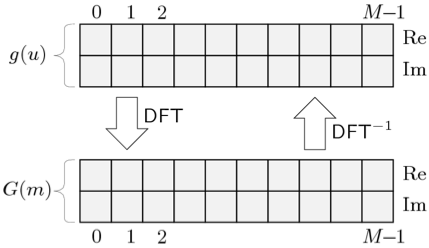
\includegraphics[scale=0.3]{dft.png}
		}
	\end{floatrow}
\end{figure}
\subsubsection*{Leistungsspektrum}
\begin{equation*}
	|G(m)| = \sqrt{G_{Re}^2(m) + G_{Im}^2(m)}
\end{equation*}
\subsubsection*{Phasenspektrum}
\begin{equation*}
	Pha(m) = arctan \left( \frac{G_{Im}(m)}{G_{Re}(m)} \right)
\end{equation*}
\subsubsection*{Implementation}
\begin{center}
	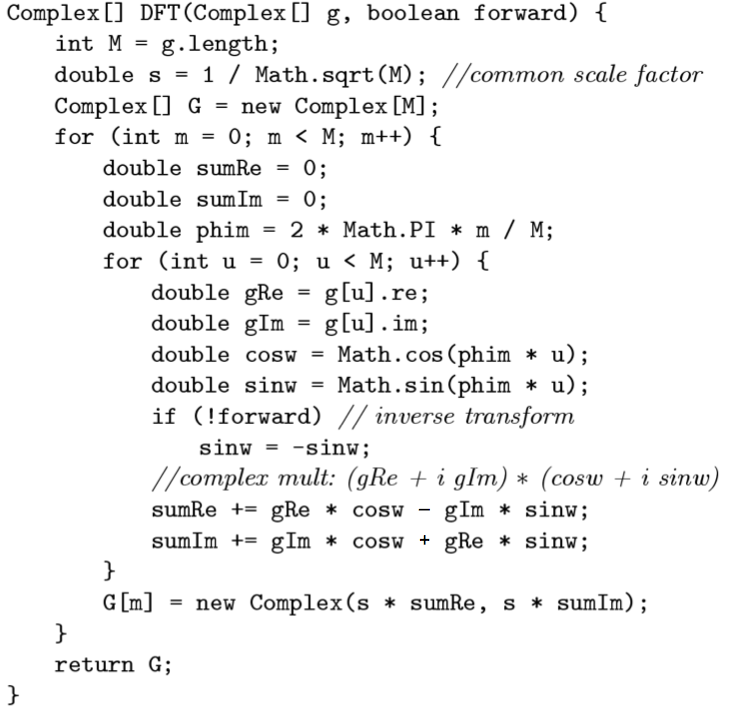
\includegraphics[scale=0.35]{dft-impl.png}
\end{center}

\subsection{FFT und DCT}
\subsubsection*{Zeitkomplexität der DFT}
\begin{itemize}
	\item zwei verschachtelte for-Schleifen von 0 bis $M$
	\item $O(M^2)$
\end{itemize}
\subsubsection*{Fast Fourier Transform (FFT)}
\begin{itemize}
	\item z.B. Algorithmus von Cooley und Tukey
	\item Optimierung auf Signallängen von $M=2^k$
	\item Reduktion der Zeitkomplexität auf $O(M \cdot log M)$
\end{itemize}
\subsubsection*{Discrete Cosine Transform (DCT)}
\begin{itemize}
	\item nur für reelle Signale geeignet
	\item Spektrum ist auch reell
	\item Transformation verwendet nur Kosinusfunktionen
\end{itemize}

\subsection{DFT in 2D}
\subsubsection*{Vorwärtstransformation}
\begin{align*}
	G(m,n) &= \frac{1}{\sqrt{MN}} \cdot \sum_{u=0}^{M-1}  g(u,v) \cdot e^{-i2\pi\frac{m \cdot u}{M}} \cdot e^{-i2\pi\frac{n \cdot v}{N}} \\
	&= \frac{1}{\sqrt{MN}} \cdot \sum_{u=0}^{M-1} \sum_{v=0}^{N-1} g(u,v) \cdot e^{-i2\pi \left( \frac{m \cdot u}{M} + \frac{n \cdot v}{N}\right)} 
\end{align*}
\subsubsection*{Rücktransformation}
\begin{align*}
	g(u,v) &= \frac{1}{\sqrt{MN}} \cdot \sum_{m=0}^{M-1} \sum_{n=0}^{N-1} g(u,v) \cdot e^{i2\pi\frac{m \cdot u}{M}} \cdot e^{i2\pi\frac{n \cdot v}{N}} \\
	&= \frac{1}{\sqrt{MN}} \cdot \sum_{m=0}^{M-1} \sum_{n=0}^{N-1} g(u,v) \cdot e^{i2\pi \left( \frac{m \cdot u}{M} + \frac{n \cdot v}{N}\right)} 
\end{align*}

\subsection{Implementierung der 2D-DFT}
\begin{align*}
	G(m,n) &= \frac{1}{\sqrt{N}} \cdot \sum_{v=0}^{N-1} \underbrace{\left[ \frac{1}{\sqrt{M}} \sum_{u=0}^{M-1} g(u,v) \cdot e^{-i2\pi\frac{m \cdot u}{M}} \cdot  \right]}_{\text{1-dim. DFT der Zeile }g(\cdot,u)} \cdot e^{-i2\pi\frac{n \cdot v}{N}} 
\end{align*}
\textbf{eindimensionale DFT genügt:}
\begin{itemize}
	\item zuerst alle Zeilen eines Bildes mit der DFT transformeiren
	\item dann alle transformierten Zeilen spaltenweise mit DFT transformieren
\end{itemize}

\subsection{SD Algorithmus}
\begin{center}
	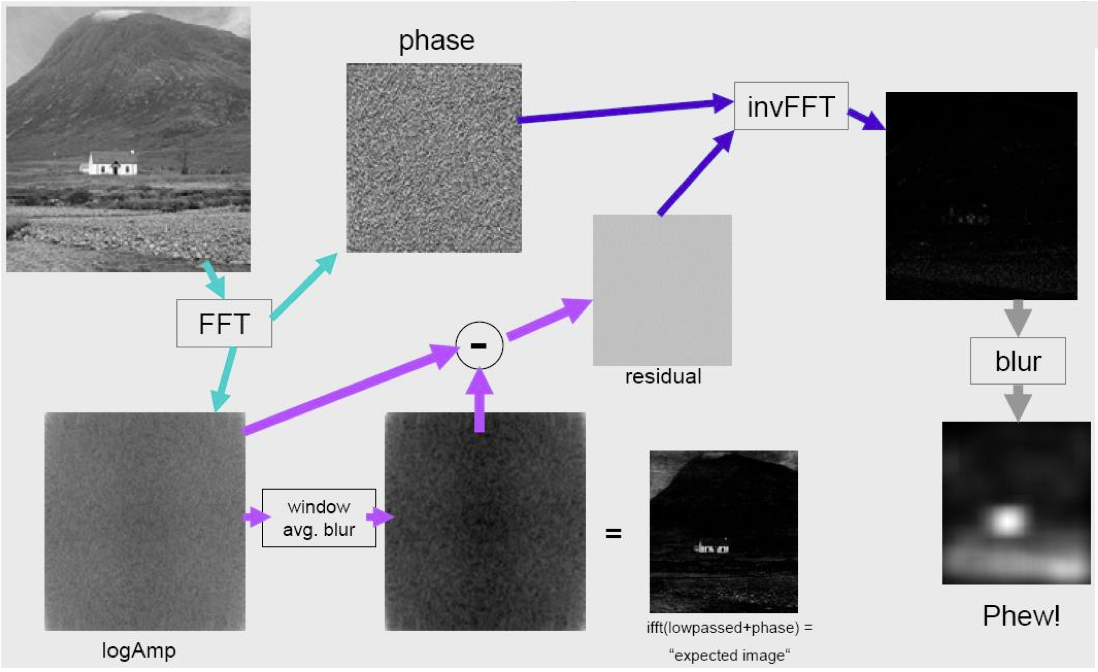
\includegraphics[scale=0.4]{sd-alg.png}
\end{center}

\pagebreak
\section{Kanten und Ecken}
\subsection{Übersicht}
\begin{description}
	\item[Gradientbasierte Kantendetektion] \hfill
		\begin{itemize}
			\item Faltungsoperationen basierend auf der 1. Ableitung
			\item typische Vertreter: Prewitt, Sobel
		\end{itemize}
	\item[Verfahren basierend auf der 2.Ableitung] \hfill
		\begin{itemize}
			\item verbesserte Kantenlokalisierung gegenüber der Gradientverfahren
			\item typische Vertreter: Laplacian of Gaussian
		\end{itemize}
	\item[Canny Edge Detector] \hfill
		\begin{itemize}
			\item basierend auf Gradientverfahren unter Ausnutzung der 2. Ableitung für Kantenlokalisierung
			\item gilt als eins der besten Verfahren
		\end{itemize}
	\item[Morphologische Verfahren] \hfill
		\begin{itemize}
			\item Ermittlun gder inneren oder äusseren Kontur
		\end{itemize}
\end{description}

\subsection{Gradient}
\begin{center}
	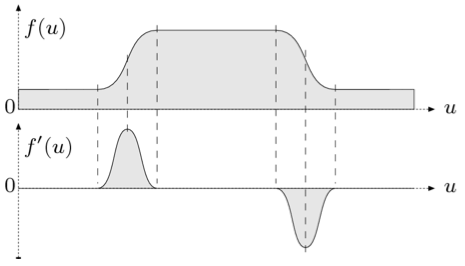
\includegraphics[scale=0.4]{ableitung.png}
\end{center}
Diskrete Approximation der Ableitung:
\begin{equation*}
	\frac{df}{du} (u) \approx \frac{f(u+1) - f(u-1)}{2} = 0.5 * (f(u+1) - f(u-1))
\end{equation*}
Partielle Ableitungen:
\begin{equation*}
	\frac{df}{du} (u, v) \hspace{2cm} \frac{df}{dv} (u, v)
\end{equation*}
Gradient:
\begin{equation*}
	\triangledown I(u,v) = \begin{bmatrix}
	\frac{df}{du} (u, v) \\ \frac{df}{dv} (u, v)
	\end{bmatrix} \hspace{2cm} | \triangledown I(u,v)  | = \sqrt{\left( \frac{df}{du} (u, v) \right)^2 + \left( \frac{df}{dv} (u, v) \right)^2}
\end{equation*}

\subsubsection{Ableitungsfilter}
Die Diskrete Approximation der ersten Ableitung lässt sich einfach mit einer diskreten Faltung realisieren:
\begin{equation*}
	\frac{df}{du} (u) \approx \frac{f(u+1) - f(u-1)}{2} = 0.5 * (f(u+1) - f(u-1)) = f(u)*\begin{bmatrix}
	-\frac{1}{2} & 0 & \frac{1}{2}
	\end{bmatrix}
\end{equation*}
Resultierende Ableitungsfilter:
\begin{align*}
	H^D_x &= \begin{bmatrix} -0.5 & \underline{0} & 0.5\end{bmatrix} = &0.5 \cdot \begin{bmatrix} -1 & \underline{0} & 1\end{bmatrix} \\
	H^D_y &= \begin{bmatrix} -0.5 \\ \underline{0} \\ 0.5\end{bmatrix} = &0.5 \cdot \begin{bmatrix} -1 \\ \underline{0} \\ 1\end{bmatrix}
\end{align*}

\subsubsection{Kantendetektierung}
Mit den Gradientfiltern $H_x$ und $H_y$ werden zwei Gradientenbilder $D_x$ und $D_y$ erzeugt. Anschliessend wird die Kantenstärke $E$ und die Kantenrichtung $\Phi$ pro Bildposition $(u, v)$ berechnet:
\begin{center}
	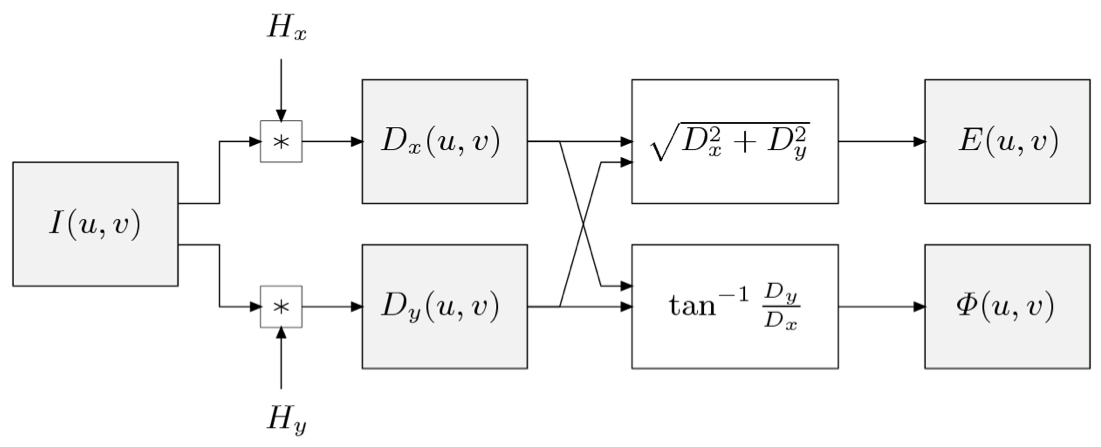
\includegraphics[scale=0.3]{gradient-dedektierung.png}
\end{center}

\subsubsection{1. und 2. Ableitung}
Problematik der Gradientenverfahren:
\begin{itemize}
	\item detektierte Kanten sind so breit wie die Steigerungsverläufe
	\item schlechte Kantenlokalisierung
\end{itemize}
Mit der Verwendung der zweiten Ableitung können die Übergänge zwischen verschiedenen Steigerungsverläufen detektiert werden:
\begin{center}
	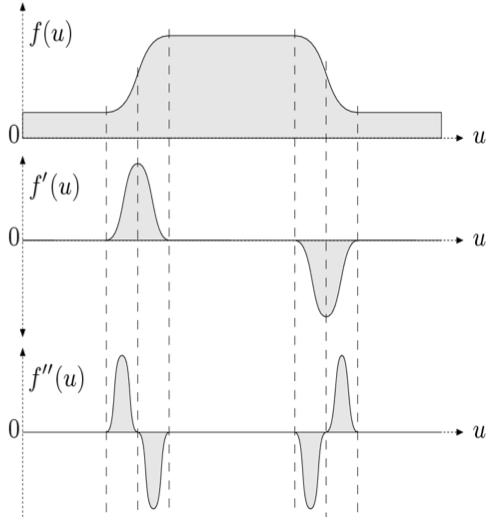
\includegraphics[scale=0.3]{2ableitung.png}
\end{center}

\subsection{Laplacian of Gaussian}
Grundidee:
\begin{itemize}
	\item Bild zuerst mit Gauss-Filter glätten (kleine scharfe Störungen verwischen)
	\item Zweite Ableitung des geglätteten Bildes bestimmen
	\item Pder: Bild mit 2. Ableitung von Gauss falten
\end{itemize}
Gauss-Funktion:
\begin{equation*}
	G_\sigma(x,y) = e^{-\frac{x^2+y^2}{2\sigma^2}}
\end{equation*}
1. partielle Ableitung:
\begin{equation*}
	\frac{\partial G(x,y)}{\partial x} = - \frac{x}{\sigma^2}e^{-\frac{x^2+y^2}{2\sigma^2}} = - \frac{x}{\sigma^2}G(x,y)
\end{equation*}
2. partielle Ableitung:
\begin{equation*}
	\frac{\partial^2 G(x,y)}{\partial^2 x} = - \frac{x^2 - \sigma^2}{\sigma^4}G(x,y)
\end{equation*}
LoG:
\begin{equation*}
	-\triangledown^2 G(x,y) = - \frac{\partial^2 G(x,y)}{\partial^2 x} - \frac{\partial^2 G(x,y)}{\partial^2 y} 
\end{equation*}

\subsubsection{Kantenschärfung}
Verwendung des Laplace-Operators:
\begin{equation*}
	(\triangledown^2 f)(x,y) = \frac{\partial^2 f(x,y)}{\partial^2 x} + \frac{\partial^2 f(x,y)}{\partial^2 y} 
\end{equation*}
Approximation der 2. Ableitungen:
\begin{equation*}
	\frac{\partial^2f}{\partial^2x} \approx H^L_x = \begin{bmatrix} 1 & \underline{-2} & 1\end{bmatrix}
	\hspace{2cm}
	\frac{\partial^2f}{\partial^2y} \approx H^L_y = \begin{bmatrix} 1 \\ \underline{-2} \\ 1\end{bmatrix}
\end{equation*}
Laplace-Filter:
\begin{equation*}
	H^L=H^L_x + H^L_y = \begin{bmatrix}
	0 & 1 & 0 \\
	1 & \underline{-4} & 1 \\
	0 & 1 & 0
	\end{bmatrix}
\end{equation*}
Kantenschärfung:
\begin{equation*}
	I' \leftarrow I - \omega \cdot (H^L * I)
\end{equation*}

\subsubsection{Anwendung des Laplace-Filters}
\begin{center}
	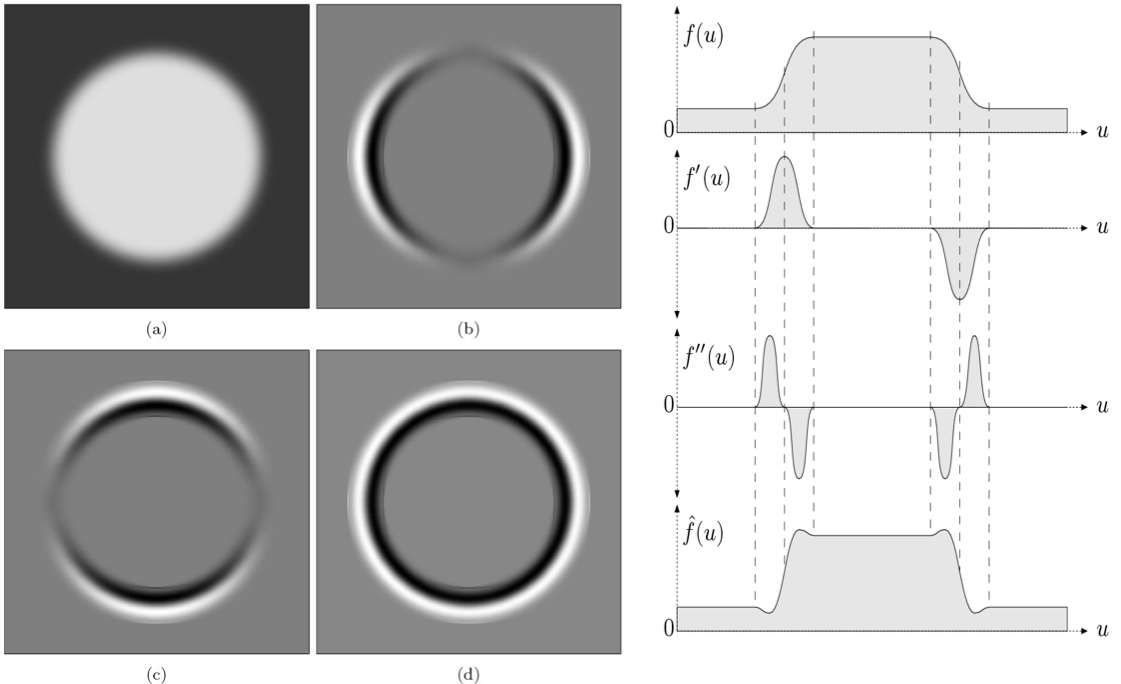
\includegraphics[scale=0.3]{laplace-filter.png}
\end{center}

\subsection{Eckpunkte}
Eckpunkte weisen Intensiätsänderung in x- und y-Richtung auf. 
\subsubsection{Anforderungen}
\begin{itemize}
	\item lokale Einzigartigkeit
	\item invariant gegenüber linearen Abbildungen
	\item unempfindlich gegenüber Rauschen
\end{itemize}
\subsubsection{Strukturmatrix}
Autokorrelation:
\begin{equation*}
	cor(u,v) = \sum_{i,j \inf \RN} [ I(u+i,v+j) - I(u+i + \Delta u, v + j + \Delta v)]^2
\end{equation*}
Taylor-Approximation des Verschobenen Bildes pro Bildpunkt berechnen:
\begin{equation*}
	A(u,v)=I^2_x(u,v)
	\hspace{2cm} 
	B(u,v)=I^2_y(u,v)
	\hspace{2cm}
	c(u,v)= I^2_x(u,v) \cdot I^2_y(u,v)
\end{equation*}
Konzeptionell zusammengefasst zur Strukturmatrix:
\begin{equation*}
	M = \begin{pmatrix}
	I^2_x & I_xI_y \\
	I_xI_y & I^2_y
	\end{pmatrix} = \begin{pmatrix}
	A & C \\
	C & B \\
	\end{pmatrix}
\end{equation*}
Strukturmatrix glätten:
\begin{equation*}
	\overline{M} = \begin{pmatrix}
	A*H^{G,\sigma} & C*H^{G,\sigma} \\
	C*H^{G,\sigma} & B*H^{G,\sigma} \\
	\end{pmatrix}= \begin{pmatrix}
	\overline{A} & \overline{C} \\
	\overline{C} & \overline{B} \\
	\end{pmatrix}
\end{equation*}
\subsubsection{Eigenwerte und Eigenvektoren}
\begin{itemize}
	\item Ein Vektor $x \neq 0$ heisst Eigenvektor einer quadratischen Matrix $A$ zum reellen Eigenwert $\lambda$, falls $Ax=\lambda x$. \\
		$(A - \lambda E)x=0$, wobei $E$ die Einheitsmatrix ist.
	\item Die Eigenwerte der MAtrix A sind alle reellen $\lambda$ für die ein Eigenvektor existiert.
	\item Die Matrix $A$ ist eine lineare Abbildung, welche den Eigenvektor $x$ nicht rotiert, sondern nur um den Faktor $\lambda$ skaliert.
	\item Wenn $A$ eine Diagonalmatrix ist, dann sind die Diagonalelemente die Eigenwerte und die Einheitsvektoren sind die Eigenvektoren.
\end{itemize}
\subsubsection{Ähnliche Matrizen}
\begin{itemize}
	\item 2 quadratische Matrizen $A$ und $D$ heissen ähnlich, falls es eine invertierbare Matrix $S$ gibt, mit $A=S^{-1}DS$
	\item eine quadratische Matrix $A$ heisst symmetrisch falls $A^T=A$
	\item Jede symmetrische Matrix $A$ ist ähnlich zu einer Diagonalmatrix $D$.  Die Diagonalelemente der Diagonalmatrix $D$ sind die Eigenwerte von $A$.
	\item Die Transformationsmatrix $S$ wird aus den orthonormierten Eigenvektoren $x_i$ gebildet, $S = [x_1,x_2, \dots, x_n]$
\end{itemize}
\subsubsection{Diagonalisierte Strukturmatrix}
Ähnliche Matrix zur geglätteten Strukturmatrix:
\begin{itemize}
	\item die Diagonalelemente sind gleich den Eigenwerten $\lambda$ \\
	$\overline{M}' = \begin{pmatrix}
	\lambda_1 & 0 \\
	0 & \lambda_2
	\end{pmatrix}$
\end{itemize}
Generelle Interpretation:
\begin{itemize}
	\item Matrix entspricht einer linearen Abbildung basierend auf einem Koordinatensystem
	\item durch geschickte Variation des Koordinatensystems kann die Abbildungsmatrix vereinfacht (diagonalisiert) werden
	\item die Eigenvektoren entsprechen den Einheitsvektoren des neuen Koordinatensystems
\end{itemize}
\subsubsection{Spezifische Interpretation}
\textbf{Eigenwerte:}
\begin{equation*}
	\lambda_{1,2} = \frac{trace(\overline{M})}{2} \pm \sqrt{\left( \frac{trace(\overline{M})}{2} \right)^2 - det(\overline{M})} = \frac{1}{2} \left( \overline{A} + \overline{B} \pm \sqrt{\overline{A}^2 - 2 \overline{A} \overline{B} + \overline{B}^2 + 4 \overline{C}^2} \right)
\end{equation*}
\begin{itemize}
	\item beide sind null in flachen Bildregionen
	\item bei einer Kante in beliebiger Richtung ist der kleinere der beiden Eigenwerte fast null
	\item nur bei Eckpunkten sind beide Eigenwerte gross
\end{itemize}
\textbf{Eigenvektoren:}
\begin{itemize}
	\item geben die Richtung der Kanten an
\end{itemize}
\subsubsection{Corner Response Function (CRF)}
Die Differenz der Eigenwerte kann als Gütemass für einen Eckpunkt gewertet werden: je kleiner die Differenz, desto eher ist es einen Eckpunkt:
\begin{equation*}
	\lambda_1 - \lambda_2 = 2 \cdot \sqrt{\frac{1}{4} \cdot \left( trace(\overline{M})'2 - det(\overline{M}) \right)}
\end{equation*}
CRF:
\begin{equation*}
	Q(u,v) = det(\overline{M}) - \alpha \cdot (trace(\overline{M})^2 = (\overline{AB} - \overline{C}^2) - \alpha \cdot (\overline{A} + \overline{B})^2
\end{equation*}
\begin{itemize}
	\item mit dem Parameter $\alpha$ wird die Empfindlichkeit gesteuert (z.B. 0.05)
	\item $Q(u,v) >$ Schwellwert (z.B. 10'000 bis 1 Mio)
\end{itemize}
\subsection{Harris Algorithmus}
\begin{center}
	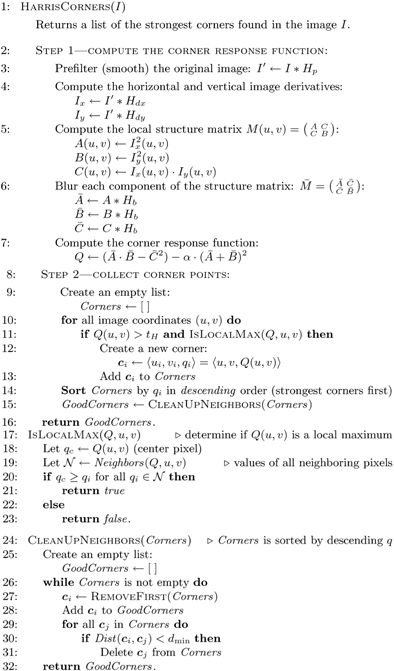
\includegraphics[scale=0.5]{harris.png}
\end{center}

\pagebreak
\section{Wavelet-Transformation}

\subsection{Einsatz der WT}
\textbf{Datenverdichtung:}
\begin{itemize}
	\item Bilder: JPEG2000, PGF, MPEG-4
	\item Audio
\end{itemize}
\textbf{Multi Resolution Models:}
\begin{itemize}
	\item Daten in verschiedenen Auflösungsstufen zur Verfügung stellen
	\item alle Auflösungsstufen in einem Kompakten Format zusammenhalten
	\item keine disjunkten Datensätze, sondern alle Daten werden benötigt, um die höchste Auflösungsstufe zu rekonstruieren
\end{itemize}

\subsection{Idee der Bildpyramide}
\begin{center}
	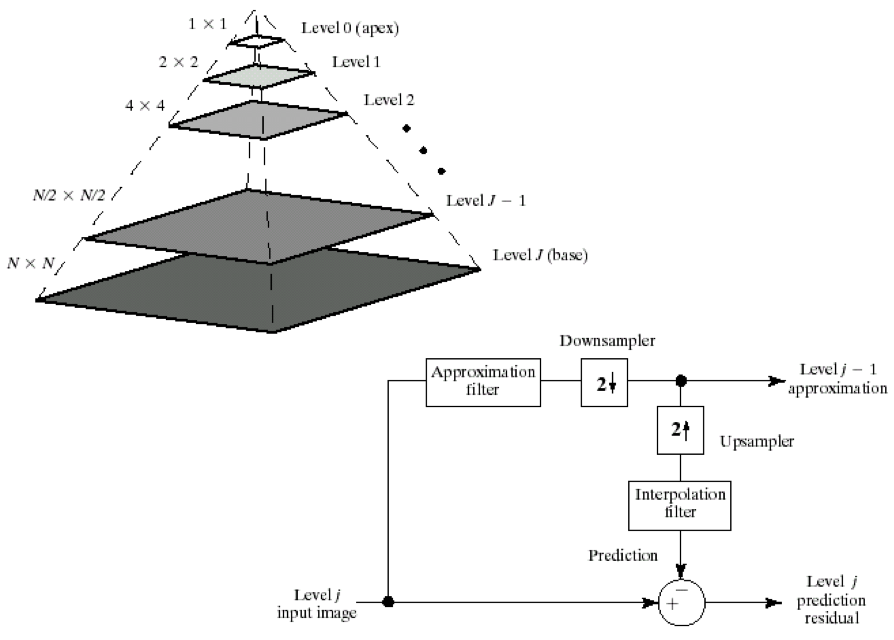
\includegraphics[scale=0.4]{wt-bildpyramide.png}
\end{center}

\subsection{$L_2$-Norm}
Ist eine Vektornorm:
\begin{equation*}
	x = \begin{bmatrix} x_1 \\ x_2 \\ \vdots \\ x_n \end{bmatrix} 
	\hspace{2cm}
	|x| = \sqrt{\sum_{k=1}^n |x_k|^2}
\end{equation*}
Ist eine Norm für Funktionen $\Phi(x)$:
\begin{equation*}
	||\Phi||^2 \equiv \Phi \circ \Phi \equiv \langle \Phi | \Phi \rangle \equiv \int |\Phi(x)|^2 dx
\end{equation*}

\subsection{Mother Wavelet und Wavelet-Familien}
Aus Mother Wavelets, auch Basis-Wavelets genannt, kann durch Skalierung ($a > 0$) und Verschiebung ($b$) eine ganze Wavelet-Familie erzeugt werden:
 \begin{equation*}
	\Psi_{a,b}(x)= \frac{1}{\sqrt{a}} \Psi \left(\frac{x-b}{a} \right)
\end{equation*}
\begin{center}
	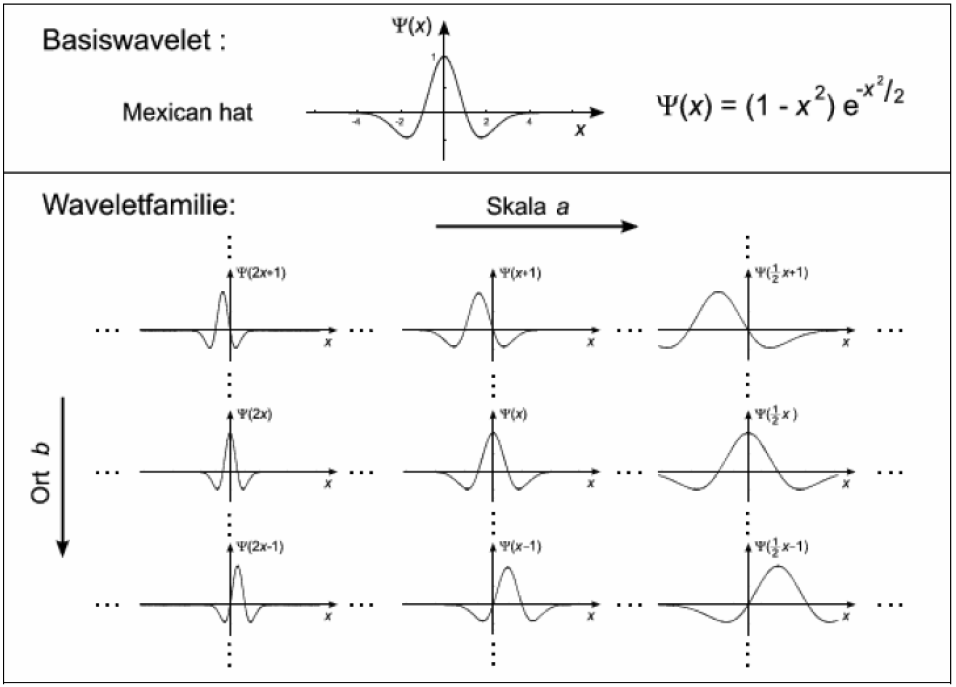
\includegraphics[scale=0.4]{wavelet-family.png}
\end{center}

\subsection{Continuous Wavelet Transform}
\begin{itemize}
	\item Ausgangssignal $f(x)$
	\item wähle beliebiges Wavelet $\Psi$
	\item berechne Skalarprodukt von $\Psi_{a,b}$ mit $f(x)$ für alle möglichen Paare von $a$ und $b$
	\item die berechneten WErte sind die Wavelet-Koeffizienten $CWT_{a,b}$
\end{itemize}
\subsubsection*{Vorwärtstransformation}
 \begin{equation*}
	CWT_{a,b}(f)=\langle f(x) | \Psi_{a,b} \rangle \equiv \int_{-\infty}^\infty f(X) \overline{\Psi_{a,b}(x)} dx
\end{equation*}
\subsubsection*{Rücktransformation}
 \begin{equation*}
	f(x)=\langle CWT_{a,b}(f) | \Psi_{a,b} \rangle \equiv \int_{\RN^*\times \RN} CWT_{a,b}(f) \overline{\Psi_{a,b}(x)} \frac{dadb}{|a|^2}
\end{equation*}

\subsection{CWT, DWT und FWT}
Problem der CWT:
\begin{itemize}
	\item es gibt unendliche viele Parameterpaare (a,b)
	\item es ist unklar, welche Parameterpaare (a,b) erforderlich sind, um eine vollständige Rekonstruktion zu ermöglichen
\end{itemize}
Lösungsansatz DWT:
\begin{itemize}
	\item üblicherweise sind diskrete Signale mit begrenzter Abtastung gegeben
	\item für diskrete Signale muss eine endliche Zahl von PArameterpaaren (a,b) ausreichen, so dass eine Rücktransformation ohne Verlust möglich ist \\
		$\rightarrow$ Discrete Wavelet Transform (DWT)
\end{itemize}
Durchbruch: FWT:
\begin{itemize}
	\item Multiresolution Analysis führte zum Algorithmus der schnellen DWT $\rightarrow$ Fast Wavelet Transform (FWT)
\end{itemize}

\subsection{FWT}
\begin{center}
	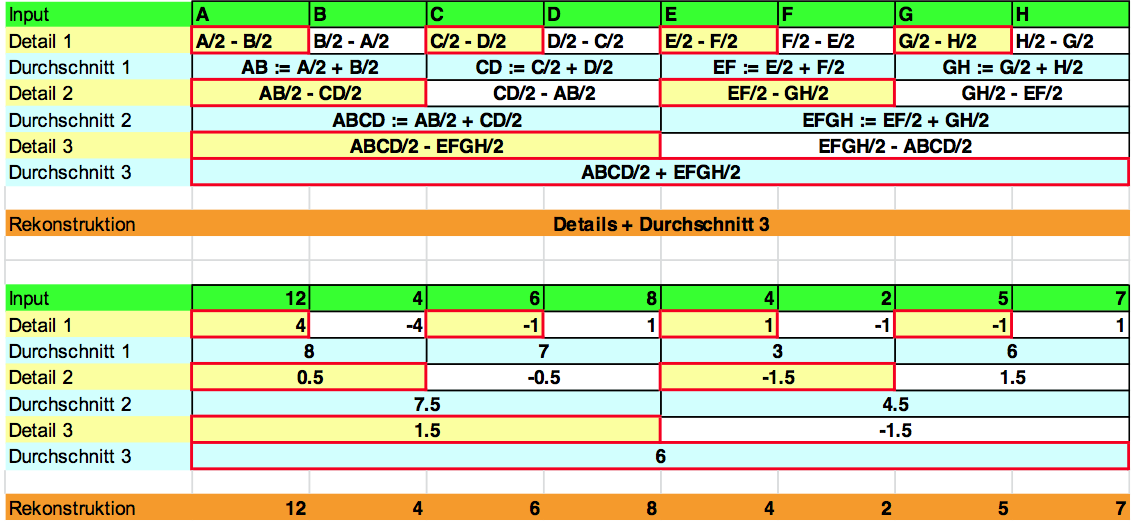
\includegraphics[scale=0.4]{fwt.png}
\end{center}

\subsection{FWT als Filteroperation}
\begin{center}
	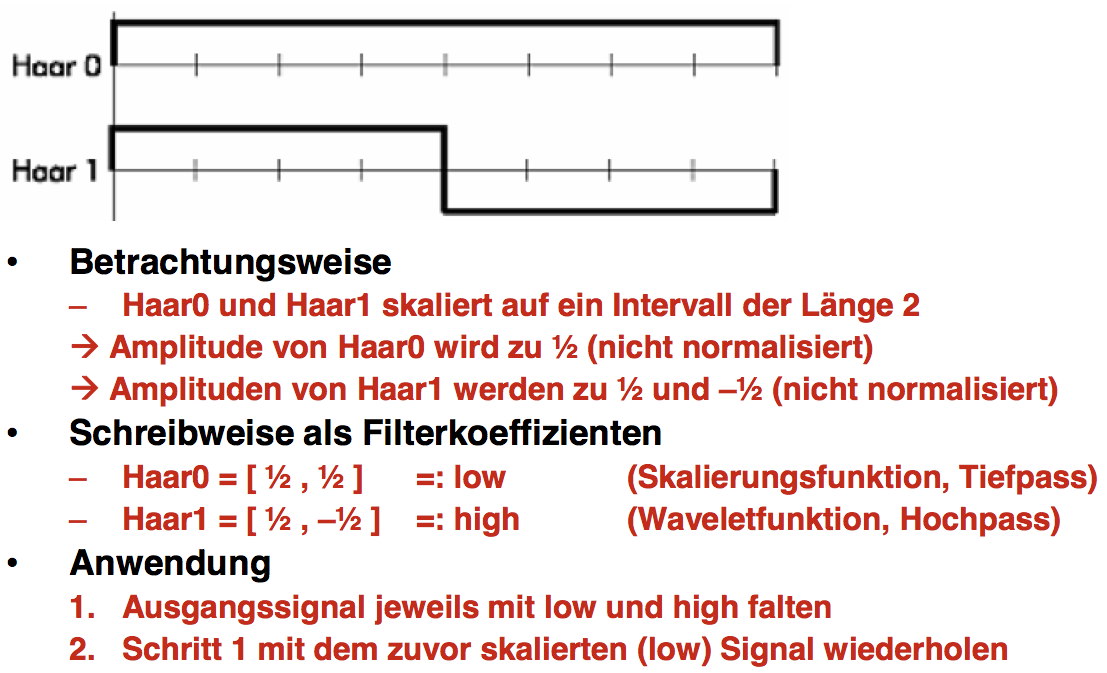
\includegraphics[scale=0.3]{fwt-filter.png}
\end{center}

\subsection{Rücktransformation}
Generelle Rekonstruktion des Ausgangssignals:
\begin{itemize}
	\item im Wesentlichen wieder ein Skalaprodukt mit einem Wavelet
	\item Analyse- und Synthese-Wavelet müssen nicht identisch sein
\end{itemize}
Bei der FWT:
\begin{itemize}
	\item Verwendung eines Synthese-Filterpaares, passend zum Analyse-Filterpaar und Anwendung der Faltung
\end{itemize}

\subsection{FWT Filterbank}
Bi-orthogonale Filterbank:
\begin{itemize}
	\item $(h_L, h_H)$: Filterpaar der Vorwärtstransformation (Low, High)
	\item $(g_L, g_R)$: Filterpaar der Rückwärtstransformation (Left, Right)
	\item Rücktransformationsfilter können aus der Vorwärtstranformationsfilter abgeleitet werden: \\
		$\langle h_L | g_R \rangle = 0$ und $\langle h_H | g_L \rangle = 0$
\end{itemize}

\subsubsection*{Beispiel}
\begin{center}
	\includegraphics[scale=0.2]{daubechies1.png}
	\includegraphics[scale=0.1]{daubechies2.png}
\end{center}

\subsection{FWT in zwei Dimensionen}
Die Grundidee ist wie bei der DFT wird für mehrere Dimensionen auf die eindimensionale Transformation zurückgegriffen. Die Filterpaare müssen auch normalisiert wein ($L_2-Norm = 1$) \\
\textbf{Standard Dekomposition:}
\begin{itemize}
	\item mehrstufige FWT für jede Zeile des Bildes
	\item mehrstufige FWT für jede Spalte des zeilentransformierten Bildes
\end{itemize}
\textbf{Nicht-Standard Dekomposition:}
\begin{itemize}
	\item 1 Filterschritt für jede Zeile eines Bildes durchführen
	\item 1 Filterschritt für jede Spalte des zeilentranformierten Bildes \\
		$\rightarrow$ vier Quadranten entstehen: LL, HL, LH, HH
	\item rekursiv den Quadranten LL wieder filtern
\end{itemize}
\begin{center}
	\includegraphics[scale=0.15]{2d-fwt-dekompositionen.png}
\end{center}

\subsection{Bilddaten-Dekorrelation}
Innerhalb eines Farbkanals gibt es noch weitere Redundanz (z.B. Flächen mit gleicher Farbe). Um die Redundanz zu reduzieren findet eine Transformation vom Bild- in den Frequenzraum statt. \\
\textbf{DCT (discrete cosine transform):}
\begin{itemize}
	\item schnell, einfach
	\item Blockbildung
	\item Einsatz in JPEG und MPEG
\end{itemize}
\textbf{DWT (discrete wavelet transform):}
\begin{itemize}
	\item schnell, einfach
	\item keine Blockbildung
	\item verlustlose Integer-Arithmetik möglich
	\item Einsatz in PGF, JPEG 2000, MPEG-4
\end{itemize}

\subsection{Quantisierung}
\textbf{Ziel:}
\begin{itemize}
	\item möglichst kleine Anzahl von unterschiedlichen Wavelet-Koeffizienten
	\item Koeffizienten mit kleinen Absolutwerten (viele Nullen)
\end{itemize}
\textbf{Ansatz:}
\begin{itemize}
	\item Zusammenfassen von ähnlich grossen Wavelet- Koeffizienten in Gruppen $\rightarrow$ Quantisierung
	\item anstatt des Wertes eines Wavelet-Koeffizienten wird seine Gruppennummer abgespeichert
	\item für jede Gruppe muss die Spannweite abgespeichert werden $\rightarrow$ Quantisierungstabelle
	\item je Grösser die Spannweite einer Gruppe, desto grösser der Informationsverlust $\rightarrow$ ohne Quantisierung kein Informationsverlust
\end{itemize}

\pagebreak
\section{PGF}
\subsection{Features}
\begin{itemize}
	\item sehr hohe verlustlose Kompressionsrate
	\item sehr gute verlustbehaftete Bildqualität/Kompressionsrate
	\item kontinuierlicher Datenstrom erlaubt schrittweise Erhöhung der Auflösung
\end{itemize}
\subsection{Aufbau}
\begin{center}
	\includegraphics[scale=0.3]{pgf-aufbau.png}
\end{center}
\subsection{Farbtransformation}
\begin{center}
	\includegraphics[scale=0.3]{pgf-farbtransformation.png}
\end{center}
\subsection{5/3 Wavelet Filterbank}
\begin{itemize}
	\item kann ganzzahlig implementiert werden, obwohl Faktor $\sqrt{2}$ vorkommt
	\item ist reletiv kurz ( kleine Anzahl von Filterkoeffizienten)
	\item gehört zu den besten Filtern für Bildverarbeitung
\end{itemize}
\subsection{Skalare Quantisierung}
\begin{center}
	\includegraphics[scale=0.2]{pgf-skalare-quantisierung.png}
\end{center}
\subsection{Progressive Kodierung}
\textbf{Ziele:}
\begin{itemize}
	\item eingebunder Bitstrom fürs sequentielles LEsen
	\item schnelles, progressives Kodierungsschema
	\item gute Komprimierungsrate
\end{itemize}
\textbf{Ansatz:}
\begin{itemize}
	\item Wavelet-Koeffizienten getrennt nach Level abspeichern
	\item Umordnen der Wavelet-Koeffizienten, so dass Koeffizienten mit ähnlich grossen Absolutwert nahe beieinander liegen
\end{itemize}
\begin{center}
	\includegraphics[scale=0.2]{pgf-dateistruktur.png}
\end{center}
\textbf{Umordnen der Koeffizienten:}
\begin{center}
	\includegraphics[scale=0.3]{pgf-koeffizienten.png}
\end{center}
\subsection{Bitplane-Kodierung}
\begin{center}
	\includegraphics[scale=0.2]{pgf-bitplane-coding.png}
\end{center}
\subsection{Lauflängenkodierung (RLE)}
\begin{center}
	\includegraphics[scale=0.25]{pgf-lauflaengencoding.png}
\end{center}
\subsection{Adaptives RLE}
\textbf{Problem:}
\begin{itemize}
	\item der bestmögliche Wert für $k$ hängt vom Input ab
	\item wird $k$ zu gross gewählt, so werden zu vilee Bits verschwendet, um $n$ abzuspeichern
	\item wird $k$ zu klein gewählt, so werden zu viele Codworte erzeugt
\end{itemize}
\textbf{Ansatz (adaptiv):}
\begin{itemize}
	\item $k$ nach jedem Codewort anpassen
	\item $k$ mit 0 initialisieren
	\item nach einem Codewort 0: $k++$
	\item nach einem anderem Codewort: $k-- (k>0)$
\end{itemize}
\section{Uebungen}
\subsection{Uebung 1}
Gegeben ist das Bild Schlittentest.raw der Grösse 800 mal 600 Bildpunkte. Es enthält einen
Header der Länge 1 KiByte in einem proprietären Format und die Bildinformation von einem
CMOS-Bildsensor mit Bayer-Maske. Pro Bildpunkt (Pixel) ist jeweils nur eine der drei Farb-
komponenten (Rot, Grün, Blau) in einem Byte abgespeichert. Die an der ersten Stelle des
Bildes gegebene Farbkomponente ist Blau. Sie können dieses Bild in ImageJ mit Fi-
le/Import/Raw öffnen.\\
Ergänzen Sie das ImageJ-Plugin BayerMask\_.java an den entsprechenden Stellen, um die
fehlenden Farbkomponenten durch Interpolation zu erzeugen. Testen Sie Ihr Programm mit
dem Bild Schlittentest.raw. Eine gute Bayer-Mask-Interpolation sollte zu möglichst wenig
Farbartefakten (z.B. Farb-Moiré im weissen Ärmel oder bei den weissen Drähten) führen
(siehe nachfolgenden Bildausschnitt).
\lstinputlisting[caption=Bayer Mask,style=JavaStyle]{Code/BayerMask_.java}
\subsection{Uebung 2}
In dieser Aufgabe wollen wir den Huffman-Code aus Aufgabe 2 verwenden, um ein Graustu-
fenbild entropiecodiert abzuspeichern. Erweitern Sie das Plugin so, dass Sie eine Binärdatei
mittels eines ObjectOutputStreams erzeugen können. Der ObjectOutputStreams eignet
sich für die Objektserialisierung. Betrachten Sie die Methoden write und encodeImage.
a) Schreiben Sie in den Header der Datei die Breite und Höhe des Bildes. Verwenden Sie
dazu einfach zwei Integer.\\
b) Für das Decodieren der Datei wird der Code-Baum aus Aufgabe 2 wiederum benötigt.
Daher sollten Sie nach dem Header den ganzen Code-Baum serialisieren.\\
c) Zum Schluss kommen noch die codierten Bilddaten. Der Einfachheit halber können Sie
ein BitSet verwenden. Iterieren Sie durch alle Pixel des Bildes und schreiben Sie den
entsprechenden Huffman-Code jedes Pixels hintereinander ins BitSet. Anschliessend
serialisieren Sie das BitSet. Tipp: Schreiben Sie den Huffman-Code jeweils mit dem
MSB zuerst ins BitSet.\\
d) Denn dazu passenden Decoder finden Sie in Huffman\_Dec.java. Falls Sie leicht anders
vorgegangen sind, müssen Sie den Decoder unter umständen leicht anpassen.\\
e) Codieren Sie ein Graustufenbild mit Ihrem Encoder (stimmt der erwartete Speicherbedarf
mit dem wirklichen überein?) und decodieren Sie die entstandene huf-Datei mit dem De-
coder. Verwenden Sie in ImageJ den ImageCalculator, um die Differenz zwischen dem
Originalbild und dem decodierten Bild zu bestimmen.
\lstinputlisting[caption=Huffman Decodierung,style=JavaStyle]{Code/Huffman_Dec.java}
In dieser Aufgabe sollen Sie einen Huffman-Entropiecodierer als ImageJ-Plugin programmie-
ren und auf ein Graustufenbild anwenden. Als Gerüst können Sie Huffman\_Enc.java ver-
wenden. Betrachten Sie die Methode createHuffmanTree().\\
a) Bestimmen Sie zuerst die Wahrscheinlichkeiten, mit denen die einzelnen Intensitäten in
einem Graustufenbild auftreten. Verwenden Sie dazu das Histogramm.\\
b) Schätzen Sie mit Hilfe des Resultats aus a) die mittlere Codelänge und den resultieren-
den Speicherbedarf für das codierte Bild ab.\\
c) Programmieren Sie die Erzeugung des Code-Baumes und speichern Sie die einzelnen
Codewörter für die verschiedenen Intensitäten ab. Zur Erzeugung des Code-Baums eig-
net sich eine PriorityQueue<Node> besonders gut, weil damit auf sehr einfache Art die
beiden Knoten mit kleinster Wahrscheinlichkeit gefunden werden können.\\
d) Berechnen Sie die mittlere Codelänge Ihres Codes und überprüfen Sie Ihr Resultat mit
demjenigen von b).
\lstinputlisting[caption=Huffman Encodierung,style=JavaStyle]{Code/Huffman_Enc.java}
\lstinputlisting[caption=Node,style=JavaStyle]{Code/Node.java}
Die aktuelle Version von ImageJ unterstützt das PGM-Dateiformat. PGM-Dateien im ASCII-
und im Binärformat können eingelesen werden, aber beim Erstellen wird immer nur das
Binärformat verwendet.\\
a) Erstellen Sie ein neues Plugin ToPGM\_.java für 8-Bit-Grauwertbilder, welches ein Bild
als PGM-Datei im ASCII-Format abspeichert.\\
b) Wie gross ist die Kompressionsrate, wenn ein Bild im Binär- anstatt im ASCII-Format
abgespeichert wird? Schätzen Sie die Kompressionsrate für ein beliebiges Bild theore-
tisch ab. Überprüfen Sie Ihre Abschätzung an konkreten Beispielen (bridge.gif).
\lstinputlisting[caption=To PGM,style=JavaStyle]{Code/ToPGM_.java}
\subsection{Uebung 3}
Programmieren Sie den linearen Histogrammausgleich gemäss Punktoperationen Folie 22.
Verwenden Sie dazu eine Lookup-Table, die Sie als int-Array der Länge 256 für alle mögli-
chen Intensitäten im Voraus berechnen. Mit der Instanzmethode applyTable() der Klasse
ImageProcessor können Sie anschliessend die Lookup-Table auf das Bild anwenden.
\lstinputlisting[caption=Linearer Histogrammausgleich,style=JavaStyle]{Code/LinHistAusgleich_.java}
Programmieren Sie die modifizierte Gammakorrektur mit variablen Werten für Gamma und
x0 gemäss Punktoperationen Folie 27 für ein Graustufenbild. Verwenden Sie wiederum eine
Lookup-Table.
\lstinputlisting[caption=Gamma,style=JavaStyle]{Code/ModGamma_.java}
Bestimmen Sie die inverse Funktion zur modifizierten Gammakorrektur. Beachten Sie dabei,
dass der Trennwert, wo zwischen linearer und Potenzfunktion unterschieden wird, auch
angepasst werden muss.\\
Programmieren Sie die inverse modifizierte Gammakorrektur mit variablen Werten für Gam-
ma und $x_0$. Verwenden Sie wiederum eine Lookup-Table.
\lstinputlisting[caption=Gamma Inverse,style=JavaStyle]{Code/ModGammaInverse_.java}
\subsection{Uebung 5}
Basierend auf der YUV-Farbtransformation der Aufgabe 1 wollen wir eine Umwandlung in ein
Grauwertbild vornehmen. Als Grauwert werden wir den Luminanzwert des YUV-Farbraums
verwenden.\\
Gegeben sei wiederum eine Eingabebild im sRGB-Farbraum mit einem effektiven Gamma $\gamma$ von 1/2.2.
a) Überführen Sie das nicht-lineare sRGB-Bild in den linearen RGB-Farbraum mit Hilfe der
modifizierten Gammakorrektur.\\
b) Erstellen Sie ein erstes Grauwertbild, indem Sie den Y-Kanal der YUV-Transformation
aus Aufgabe 1 berechnen.\\
c) Eine abgekürzte, nicht ganz korrekte Umrechnung erlaubt die Transformation in einem
einzigen Schritt aus den sRGB-Komponenten. Dabei wird Y wie folgt berechnet:
$Y = 0.309*R’ + 0.609*G’ + 0.082*B’$\\
d) Bestimmen Sie die Bildqualität des zweiten Grauwertbildes bezüglich des ersten in dB.
Berechnen Sie dazu die PSNR.
\lstinputlisting[caption=RGB zu Graustufenbild,style=JavaStyle]{Code/RGBtoGray_.java}
YUV ist die Basis für die Farbkodierung im analogen Fernsehen, sowohl im nordamerikani-
schen NTSC- als auch im europäischen PAL-System. Die Luminanzkomponente Y wird aus
den RGB-Komponenten in der Form\\
$Y = 0.299*R + 0.587*G + 0.114*B$\\
abgeleitet, wobei angenommen wird, dass die RGB-Werte bereits nach dem TV-Standard für
die Wiedergabe gammakorrigiert sind ($\gamma NTSC = 2.2$). Die UV-Komponenten sind als gewichte-
te Differenz zwischen dem Luminanzwert und dem Blau- bzw. Rotwert definiert, konkret als
$U = 0.492*(B – Y)$\\
 und\\
 $V = 0.877*(R – Y)$.\\
a) Programmieren Sie die lineare RGB-YUV-Farbtransformation für das amerikanische
Fernsehsystem NTSC. Das Eingabebild sei im nicht-linearen sRGB-Farbraum mit einem
effektiven Gamma $\gamma$ von 1/2.2.\\
b) Programmieren Sie die lineare YUV-RGB-Rücktransformation. Die Koeffizienten der
Rücktransformationsmatrix erhalten Sie durch Inversion der Matrix.\\
c) Berechnen Sie die Qualität des rücktransformierten Bildes bezüglich des Originals. Be-
rechnen Sie dazu die PSNR für jeden der drei Farbkanäle.
\lstinputlisting[caption=YUV Transformation,style=JavaStyle]{Code/YUVTransform_.java}
\subsection{Uebung 6}
Implementieren Sie ein Gauss’sches Glättungsfilter. Die Grösse des Filters (Radius $\sigma$) soll
beliebig einstellbar sein. Ein sinnvoller Wert von $\sigma$ wäre zum Beispiel 3. Erstellen Sie die
zugehörige Filtermatrix dynamisch mit einer Grösse von mindestens 5$\sigma$ in beiden Richtun-
gen. Nutzen Sie die x-/y-Separierbarkeit der Gaussfunktion.
\lstinputlisting[caption=Gauss Filter,style=JavaStyle]{Code/GaussFilter_.java}
Implementieren Sie ein gewichtetes Medianfilter. Spezifizieren Sie die Gewichte als konstan-
tes, zweidimensionales Integer-Array. Testen Sie das Filter und vergleichen Sie es mit einem
gewöhnlichen Medianfilter.
\lstinputlisting[caption=Gewichteter Median Filter,style=JavaStyle]{Code/GewMedianFilter_.java}
Programmieren Sie eine Prozedur zur linearen Filterung. Das Bild und die Filtermatrix sollen
dabei als Parameter übergeben werden. Zur Behebung der Randproblematik verwenden Sie
auf der einen Seite die Absolutwerte von negativen Pixelkoordinaten und auf der andern
Seite das Entsprechende.
\lstinputlisting[caption=Lineares Filter,style=JavaStyle]{Code/LinearesFilter_.java}
\subsection{Uebung 7}
Ausgehend von der Implementierung der linearen Faltung (Übung 6, Aufgabe 2.1) können
Sie auf einfache Art die Grauwert-Dilation programmieren. Erlauben Sie Strukturmatrizen
beliebiger Form, d.h. lassen Sie es zu, dass gewisse Elemente der Strukturmatrix nicht
berücksichtigt werden.
\lstinputlisting[caption=Grauwerterosion,style=JavaStyle]{Code/GrauwertDilation_.java}
Analog zu Aufgabe 1, jetzt aber für die Grauwert-Erosion.
\lstinputlisting[caption=Grauwertdilation,style=JavaStyle]{Code/GrauwertErosion_.java}
\subsection{Uebung 8}
Gegeben ist das Graustufenbild coins.png. Schreiben Sie ein Programm, welches die Anzahl
der Münzen bestimmt und jede Münze mit einer eigenen Farbe einfärbt.\\
a) Beachten Sie, dass das Graustufenbild zuerst binarisiert und allfällige Störungen elimi-
niert werden sollen, bevor Sie das Flood Filling Verfahren anwenden können. Schreiben
Sie eine Methode, die das Bild und einen Schwellwert als Input heben und ein neues Bi-
närbild generiert.\\
b) Verwenden Sie für das anschliessende Flood Filling ein effizientes Verfahren, welches
auch für grössere Bilder geeignet ist.\\
c) Erzeugen Sie ein neues Falschfarbenbild, welches den Hintergrund schwarz und die
Münzen in Falschfarben darstellt.
\lstinputlisting[caption=Region Labeling,style=JavaStyle]{Code/RegionLabeling_.java}
\subsection{Uebung 10}
a) Programmieren Sie die Kantendetektierung mittels verbessertem Sobel-Filtern:
\begin{equation*}
H_x = \frac{1}{32} \begin{pmatrix} -3 & 0 & 3\\-10& 0& 10\\ 	-3& 0& 3\end{pmatrix} \T{und} H_y=\frac{1}{32}\begin{pmatrix} -3&-10&-3 \\ 0&0&0 \\ 3&10&3  \end{pmatrix}
\end{equation*}\\
Geben Sie die Kantenstärke sowie die Kantenrichtung als Bilder aus.\\
Wenden Sie Ihren Kantendetektor auf windisch.png an.\\
b) Färben Sie die Kanten anhand ihrer Winkel ein und geben Sie sie in einem Bild aus.
Wählen Sie zum Beispiel die Hue-Komponente des HSV oder HLS-Farbraumes für den
winkelabhängigen Farbton.\\
Wenden Sie das angepasste Verfahren auf coins.png an.
\lstinputlisting[caption=Corner,style=JavaStyle]{Code/Corner.java}
Vervollständigen Sie das ImageJ Plugin HarrisCornerPlugin\_.java indem Sie die Corner
Response Funktion makeCrf()der Klasse HarrisCornerDetector ausprogrammieren.\\
Adaptieren Sie zudem die Zeichnungsmethode der Eckpunkte, um die Eckpunktstärke gra-
phisch darzustellen.
\lstinputlisting[caption=Harris Corner Detection,style=JavaStyle]{Code/HarrisCornerDetector.java}
\lstinputlisting[caption=Harris Corner Plugin,style=JavaStyle]{Code/HarrisCornerPlugin_.java}


\end{document} 